\documentclass[11pt,openany]{book}

\usepackage{fontspec}
\usepackage{xeCJK}
\usepackage{geometry}
\usepackage{xcolor}
\usepackage{graphicx}
\usepackage{microtype}
\usepackage{setspace}
\usepackage{titlesec}
\usepackage{fancyhdr}
\usepackage{enumitem}
\usepackage{booktabs}
\usepackage{tabularx}
\usepackage{longtable}
\usepackage{array}
\usepackage{amsmath}
\usepackage{amssymb}
\usepackage{tikz}
\usetikzlibrary{arrows.meta,positioning,fit,backgrounds,calc}
\usepackage[most]{tcolorbox}
\usepackage{xurl}
\usepackage{hyperref}
\usepackage{bookmark}

\setmainfont{Noto Sans}
\setCJKmainfont{NanumMyeongjo}
\setsansfont{Noto Sans}
\setCJKsansfont{NanumGothic}
\setmonofont{DejaVu Sans Mono}
\xeCJKsetup{CJKspace=true}
\XeTeXlinebreaklocale "ko"
\XeTeXlinebreakskip = 0pt plus 1pt

\geometry{
  paperwidth=170mm,
  paperheight=240mm,
  inner=21mm,
  outer=18mm,
  top=22mm,
  bottom=23mm,
  headheight=14pt,
  headsep=8mm
}

\definecolor{deepblue}{HTML}{102A43}
\definecolor{midblue}{HTML}{1E5A7A}
\definecolor{teal}{HTML}{1D7A73}
\definecolor{coral}{HTML}{D96C4F}
\definecolor{gold}{HTML}{C58B2A}
\definecolor{ink}{HTML}{1B242C}
\definecolor{muted}{HTML}{5C6B76}
\definecolor{paper}{HTML}{FBFAF6}
\definecolor{cream}{HTML}{F3EFE5}
\definecolor{paleblue}{HTML}{EAF2F5}
\definecolor{paleteal}{HTML}{EAF4F1}
\definecolor{palecoral}{HTML}{F9EEE9}
\definecolor{linegray}{HTML}{D9E0E3}

\pagecolor{paper}
\color{ink}
\setstretch{1.34}
\setlength{\parindent}{1em}
\setlength{\parskip}{0.42em}
\setlist[itemize]{leftmargin=1.5em,itemsep=0.25em,topsep=0.35em}
\setlist[enumerate]{leftmargin=1.7em,itemsep=0.25em,topsep=0.35em}

\hypersetup{
  colorlinks=true,
  linkcolor=midblue,
  urlcolor=teal,
  citecolor=midblue,
  pdftitle={2026 하반기 Physical AI 동향},
  pdfsubject={모델에서 운영 가능한 폐루프로},
  pdfkeywords={Physical AI, robotics, embodied intelligence, world model, VLA},
  pdfcreator={XeTeX}
}

\titleformat{\chapter}[display]
  {\sffamily\bfseries\color{deepblue}}
  {\color{coral}\fontsize{42}{42}\selectfont\thechapter}
  {-2pt}
  {\Huge}
  [\vspace{0.7em}{\color{linegray}\titlerule}]
\titlespacing*{\chapter}{0pt}{-8pt}{26pt}

\titleformat{\section}
  {\Large\sffamily\bfseries\color{deepblue}}
  {\thesection}{0.65em}{}
\titlespacing*{\section}{0pt}{1.8em}{0.7em}

\titleformat{\subsection}
  {\large\sffamily\bfseries\color{midblue}}
  {\thesubsection}{0.6em}{}
\titlespacing*{\subsection}{0pt}{1.35em}{0.5em}

\pagestyle{fancy}
\fancyhf{}
\fancyhead[LE]{\small\sffamily\color{muted}\thepage\hspace{1em}\leftmark}
\fancyhead[RO]{\small\sffamily\color{muted}\rightmark\hspace{1em}\thepage}
\renewcommand{\headrulewidth}{0.3pt}
\renewcommand{\headrule}{\hbox to\headwidth{\color{linegray}\leaders\hrule height \headrulewidth\hfill}}
\renewcommand{\chaptermark}[1]{\markboth{#1}{}}
\renewcommand{\sectionmark}[1]{\markright{#1}}

\newcommand{\keyterm}[1]{{\sffamily\bfseries\color{deepblue}#1}}
\newcommand{\eng}[1]{{\sffamily\color{midblue}#1}}
\newcommand{\watch}[2]{%
  \noindent
  \parbox[t]{0.31\linewidth}{%
    \vspace{0pt}\raggedright\sffamily\bfseries\color{teal}%
    \hyphenpenalty=10000\exhyphenpenalty=10000\strut #1\strut\par
  }%
  \hfill
  \parbox[t]{0.65\linewidth}{%
    \vspace{0pt}\raggedright\strut #2\strut\par
  }%
  \par\smallskip
}
\newcommand{\chaptertakeaway}[1]{%
  \begin{tcolorbox}[
    breakable,
    colback=deepblue,
    colframe=deepblue,
    coltext=white,
    boxrule=0pt,
    arc=2mm,
    left=5mm,right=5mm,top=4mm,bottom=4mm
  ]
  {\sffamily\bfseries\large 이 장의 한 문장}\par\smallskip
  #1
  \end{tcolorbox}
}

\newtcolorbox{profbox}[1][옆자리 해설]{
  breakable,
  enhanced,
  colback=cream,
  colframe=gold,
  boxrule=0.6pt,
  leftrule=3pt,
  arc=1.5mm,
  title={#1},
  fonttitle=\sffamily\bfseries,
  coltitle=deepblue,
  attach boxed title to top left={xshift=3mm,yshift=-2mm},
  boxed title style={colback=cream,colframe=cream},
  top=5mm,left=4mm,right=4mm,bottom=3.5mm
}

\newtcolorbox{boardbox}[1][칠판 한 장]{
  breakable,
  enhanced,
  colback=paleblue,
  colframe=midblue,
  boxrule=0.6pt,
  arc=1.5mm,
  title={#1},
  fonttitle=\sffamily\bfseries,
  coltitle=white,
  boxed title style={colback=midblue,colframe=midblue},
  attach boxed title to top left={xshift=3mm,yshift=-2mm},
  top=5mm,left=4mm,right=4mm,bottom=3.5mm
}

\newtcolorbox{fieldbox}[1][현장에서는]{
  enhanced,
  colback=paleteal,
  colframe=teal,
  boxrule=0.6pt,
  arc=1.5mm,
  title={#1},
  fonttitle=\sffamily\bfseries,
  coltitle=white,
  boxed title style={colback=teal,colframe=teal},
  attach boxed title to top left={xshift=3mm,yshift=-2mm},
  top=5mm,left=4mm,right=4mm,bottom=3.5mm
}

\newtcolorbox{cautionbox}[1][과장하지 말아야 할 지점]{
  breakable,
  enhanced,
  colback=palecoral,
  colframe=coral,
  boxrule=0.6pt,
  arc=1.5mm,
  title={#1},
  fonttitle=\sffamily\bfseries,
  coltitle=white,
  boxed title style={colback=coral,colframe=coral},
  attach boxed title to top left={xshift=3mm,yshift=-2mm},
  top=5mm,left=4mm,right=4mm,bottom=3.5mm
}

\newtcolorbox{termcard}[1]{
  breakable,
  colback=white,
  colframe=linegray,
  title={#1},
  fonttitle=\sffamily\bfseries,
  coltitle=deepblue,
  boxrule=0.5pt,
  arc=1mm,
  left=4mm,right=4mm,top=3mm,bottom=3mm
}

\newtcolorbox{pivotcard}[2]{
  breakable,
  enhanced,
  colback=white,
  colframe=linegray,
  boxrule=0.6pt,
  leftrule=4pt,
  arc=1.5mm,
  title={\textcolor{teal}{\fontsize{18}{20}\selectfont #1}\quad #2},
  fonttitle=\sffamily\bfseries\large,
  coltitle=deepblue,
  attach boxed title to top left={xshift=3mm,yshift=-2mm},
  boxed title style={colback=white,colframe=white},
  top=6mm,left=5mm,right=5mm,bottom=4mm
}

\newtcolorbox{examplebox}[1][강의실 예시]{
  breakable,
  enhanced,
  colback=white,
  colframe=gold,
  boxrule=0.6pt,
  arc=1.5mm,
  title={#1},
  fonttitle=\sffamily\bfseries,
  coltitle=deepblue,
  attach boxed title to top left={xshift=3mm,yshift=-2mm},
  boxed title style={colback=cream,colframe=gold},
  top=5mm,left=4mm,right=4mm,bottom=3.5mm
}

\newtcolorbox{translationbox}[1][한 문장 번역]{
  breakable,
  enhanced,
  colback=deepblue,
  colframe=deepblue,
  coltext=white,
  boxrule=0pt,
  arc=1.5mm,
  title={#1},
  fonttitle=\sffamily\bfseries,
  coltitle=white,
  attach boxed title to top left={xshift=3mm,yshift=-2mm},
  boxed title style={colback=coral,colframe=coral},
  top=5mm,left=5mm,right=5mm,bottom=4mm
}

\newcommand{\sourceitem}[3]{%
  \par\smallskip\noindent
  {\sffamily\bfseries\color{deepblue}#1}\par
  {\footnotesize #2\par\href{#3}{\nolinkurl{#3}}}\par
}

\begin{document}
\frontmatter

\begin{titlepage}
\pagecolor{deepblue}\color{white}
\thispagestyle{empty}
\vspace*{14mm}

{\sffamily\bfseries\fontsize{15}{18}\selectfont
2026년 7월까지의 공개 기술 변화로 읽는\par}
\vspace{11mm}

{\sffamily\bfseries\fontsize{32}{40}\selectfont
2026 하반기\par
Physical AI 동향\par}

\vspace{8mm}
{\color{coral}\rule{45mm}{2.5pt}}\par
\vspace{8mm}

{\sffamily\fontsize{17}{25}\selectfont
모델이 몸을 얻은 뒤,\par
무엇이 달라지는가\par}

\vfill

\begin{minipage}{0.82\textwidth}
\color{white!84}
\large
인지하고, 기억하고, 계획하고, 움직인 뒤 다시 확인하는 시스템.\par
이 책은 Physical AI를 ``큰 모델 하나''가 아니라\par
\textbf{책임지는 폐루프}로 읽는 해설서다.
\end{minipage}

\vspace{18mm}
{\sffamily\small 2026년 하반기 전망판 \quad\textbullet\quad 추가 강의 수록 \quad\textbullet\quad 2026년 7월 26일 기준}
\end{titlepage}

\pagecolor{paper}\color{ink}
\cleardoublepage

\chapter*{이 책을 펼치기 전에}
\addcontentsline{toc}{chapter}{이 책을 펼치기 전에}

로봇이 컵을 정확히 알아봤다고 해봅시다. 지시도 알아들었고, 팔도 움직였습니다. 그런데 컵을 떨어뜨렸다면 우리는 그 로봇의 인식이 성공했다고 말해야 할까요? 디지털 AI에서는 좋은 답을 내놓는 일이 결과의 끝인 경우가 많습니다. Physical AI에서는 출력이 환경을 바꿉니다. 잘못된 답은 틀린 문장이 아니라 충돌, 파손, 정지 시간, 사람의 개입으로 이어집니다.

그래서 이 책은 모델의 이름이나 기록을 줄 세우지 않습니다. 대신 로봇 한 대를 현장에 투입한다는 사고실험을 따라갑니다. 명령을 알아듣는 일에서 시작해 공간을 재고, 접촉을 느끼고, 긴 작업을 기억하고, 미래를 상상하고, 실패를 복구하며, 여러 로봇에 업데이트를 배포하는 데까지 차례로 걸어갑니다.

\begin{profbox}
여기서 먼저 중요한 경계를 하나 그어둡시다. 이 책은 2026년 7월 26일까지 공개적으로 확인할 수 있는 기술 변화에 기초해, 하반기에 무엇을 관찰해야 하는지를 해설합니다. 하반기 전체를 이미 일어난 사실처럼 서술하지 않습니다. ``확산될 것이다''라고 단정하기보다, 어떤 조건이 충족되면 그 방향이 강해지는지와 어떤 숫자가 전망을 뒤집는지를 함께 적습니다.
\end{profbox}

이 책의 중심 명제는 간단합니다.

\begin{quote}
\large\itshape
2026년의 중요한 변화는 더 큰 모델의 등장이 아니라, 인지--기억--계획--행동--검증--복구가 하나의 실행 루프로 연결되기 시작했다는 점이다.
\end{quote}

좋은 엔진 하나가 좋은 항공기를 만들지 못합니다. 엔진, 조종계통, 항법, 경보, 정비 체계가 연결되어야 비행이 됩니다. Physical AI도 이제 ``엔진 시연''에서 ``항공기 조립''으로 넘어가는 중입니다. 이 비유를 기억하면 뒤에 나오는 VLA, 월드모델, 메모리, 3D 표현, 촉각, 런타임 검증 같은 용어들이 각자 어디에 놓이는지 훨씬 잘 보일 것입니다.

\section*{읽는 법}

각 장에는 네 종류의 해설 상자가 반복됩니다.

\begin{itemize}
  \item \keyterm{옆자리 해설}: 흔히 생기는 오해를 교수의 구두 설명처럼 바로잡습니다.
  \item \keyterm{칠판 한 장}: 구조, 수식, 시간척도를 한눈에 정리합니다.
  \item \keyterm{현장에서는}: 논문의 성능이 지연, 안전, 정비비, 사람 개입으로 어떻게 번역되는지 봅니다.
  \item \keyterm{하반기에 볼 숫자}: 전망을 믿거나 버리기 위해 실제로 확인할 지표를 제시합니다.
\end{itemize}

\begin{cautionbox}
공개된 기술 보고서와 프로젝트 페이지는 최신 방향을 읽는 데 유용하지만, 독립적인 재현을 모두 보장하지는 않습니다. 기업 발표의 수치는 해당 팀의 조건에서 보고된 결과로 읽고, 분야 전체의 보편적 성능으로 일반화하지 않습니다. 또한 산업용 로봇 안전 표준이나 AI 규정의 적용 범위는 제품과 용도에 따라 다르므로, 특정 문서가 모든 로봇을 자동으로 규율한다고 해석해서는 안 됩니다.
\end{cautionbox}

\tableofcontents
\cleardoublepage

\mainmatter

\chapter{왜 지금 Physical AI인가}
\chaptertakeaway{질문이 ``로봇이 할 수 있는가''에서 ``반복해서 맡겨도 되는가''로 바뀌고 있다.}

\section{지능이 화면 밖으로 나오는 순간}

디지털 모델은 틀리면 다시 생성할 수 있습니다. 로봇은 한 번의 잘못된 행동으로 대상의 위치를 바꾸고, 다음 입력까지 바꿉니다. 바로 이 점 때문에 Physical AI는 \keyterm{폐루프 시스템}입니다. 관측이 행동을 만들고, 행동이 세계를 바꾸며, 바뀐 세계가 다음 관측이 됩니다.

그동안 로봇 연구의 많은 성과는 각각의 부품에서 나왔습니다. 카메라는 물체를 더 잘 찾았고, 언어 모델은 복잡한 지시를 해석했으며, 정책은 시연된 동작을 더 자연스럽게 재현했습니다. 문제는 부품의 성능을 더한다고 시스템의 신뢰성이 자동으로 생기지 않는다는 데 있습니다. 인식이 맞아도 좌표가 틀릴 수 있고, 계획이 맞아도 모터 명령이 늦을 수 있으며, 한 단계의 작은 오차가 긴 작업에서 누적될 수 있습니다.

\begin{boardbox}[폐루프를 이루는 일곱 역할]
\centering
\begin{tikzpicture}[
  node distance=4.3mm and 4.8mm,
  every node/.style={font=\sffamily\small,align=center},
  role/.style={draw=midblue,rounded corners=1.5mm,fill=white,minimum width=20mm,minimum height=10mm},
  arr/.style={-{Latex[length=2mm]},thick,color=teal}
]
\node[role] (sense) {관측};
\node[role,right=of sense] (state) {세계 상태};
\node[role,right=of state] (memory) {기억};
\node[role,below=of memory] (plan) {추론·계획};
\node[role,left=of plan] (policy) {정책};
\node[role,left=of policy] (act) {행동};
\node[role,below=of policy,fill=palecoral,draw=coral] (verify) {검증·복구};
\draw[arr] (sense) -- (state);
\draw[arr] (state) -- (memory);
\draw[arr] (memory) -- (plan);
\draw[arr] (plan) -- (policy);
\draw[arr] (policy) -- (act);
\draw[arr] (act) -| ([xshift=-5mm]sense.west) |- (sense.west);
\draw[arr] (verify) -- (policy);
\draw[arr] (act) |- (verify);
\end{tikzpicture}
\par\medskip
\small 모델 하나가 이 역할을 모두 맡을 필요는 없다. 중요한 것은 역할 사이의 상태와 책임이 끊기지 않는 것이다.
\end{boardbox}

\section{2026년에 동시에 도착한 다섯 변화}

첫째, 시각--언어--행동을 잇는 범용 정책이 단순한 새 물체 인식을 넘어 \keyterm{새 과업의 조합}과 \keyterm{다른 기체로의 전이}를 겨냥하기 시작했습니다. 범용성의 가치는 ``말을 알아듣는다''는 데서 끝나지 않습니다. 새 작업마다 정책을 처음부터 다시 만드는 비용을 줄이는 데 있습니다.

둘째, 월드모델이 그럴듯한 영상을 만드는 생성기에서 행동의 결과를 미리 시험하는 장치로 확장되고 있습니다. 카메라 영상뿐 아니라 LiDAR 같은 센서 출력을 함께 생성하고, 후보 행동에 따른 미래를 비교하며, 희귀 상황을 통제된 방식으로 재현하려는 시도가 연결됩니다.

셋째, 메모리, 계층적 계획, 빠른 제어기, 런타임 검증기가 각자의 역할을 가진 부품으로 드러났습니다. 긴 입력창 하나로 모든 이력을 밀어 넣는 대신, 어떤 상태를 보존하고 어떤 판단을 느리게 하며 어떤 반응을 빠르게 해야 하는지가 설계 문제로 올라왔습니다.

넷째, 실제 로봇과 장기 작업을 이용한 평가가 선별된 짧은 데모와 평균 성공률의 한계를 더 분명히 보여주고 있습니다. 한 번의 성공보다 여러 환경에서의 반복 가능성, 사람 개입, 부분 성공, 복구 시간이 중요해졌습니다.

다섯째, 안전 표준과 규제 적용 일정이 인간 감독, 로그, 강건성, 사후 모니터링을 현실적인 설계 제약으로 끌어올리고 있습니다. 이것이 연구의 유일한 원인은 아니지만, 제품을 만드는 조직에는 모델 선택과 시스템 구조를 바꾸는 압력으로 작동합니다.

\begin{profbox}
자, 이 다섯 가지를 하나의 문장으로 줄여봅시다. \textbf{모델이 충분히 유능해져서, 이제는 모델 바깥의 문제가 보이기 시작했다}는 것입니다. 추론 지연, 기억 오염, 센서 보정, 실패 복구, 승인된 업데이트 경계는 예전에도 있었지만, 범용 정책이 여러 작업을 건드리기 시작하자 더 이상 주변 문제가 아니게 됐습니다.
\end{profbox}

\section{시간축으로 보는 전환}

\begin{center}
\begin{tabularx}{\textwidth}{>{\sffamily\bfseries\color{deepblue}}p{0.22\textwidth}X}
\toprule
시기 & 중심 변화 \\
\midrule
2023--2024 & 대규모 로봇 데이터 혼합, 생성형 연속 행동, 서로 다른 기체의 경험을 함께 학습하는 토대가 마련됐다. \\
2025 & 언어와 행동의 공통 인터페이스, 행동 압축, 엣지 실행, 실시간 행동 묶음, 고수준--저수준 정책 분리가 구체화됐다. \\
2026년 상반기 & 메모리, 월드모델, 런타임 검증, 현장 보정, 다중 센서 생성이 같은 실행 루프 안으로 들어오는 공개 사례가 늘었다. \\
2026년 하반기 & 통합된 스택이 실제로 오래 작동하는지, 실패를 얼마나 빨리 알아채고 복구하는지, 현장 비용을 줄이는지가 관찰 포인트다. \\
2027년 이후 & 모델 크기보다 가동률, 사람 개입, 복구, 데이터 순환, 안전 근거, 롤백이 차이를 만들 가능성이 크다. \\
\bottomrule
\end{tabularx}
\end{center}

\section{세 가지 역설}

\subsection{범용성이 커질수록 검증 범위도 커진다}

열 가지 작업만 하는 로봇보다 백 가지 작업을 하는 로봇이 매력적입니다. 그러나 가능한 상태와 실패 경로도 함께 늘어납니다. 앞으로 ``범용''이라는 주장은 가능한 작업의 수만 말해서는 부족합니다. 무엇을 거절하는지, 어느 불확실성에서 사람에게 넘기는지, 어떤 기체와 환경까지 검증했는지를 함께 제시해야 합니다.

\subsection{영상이 사실적일수록 물리 오류가 숨어들 수 있다}

월드모델이 만든 미래 장면이 눈으로 보기에 훌륭해도 접촉력, 마찰, 충돌 가능성, 인과 관계가 맞는다는 보장은 없습니다. 사람은 사실적인 장면을 쉽게 믿습니다. 그래서 생성 품질의 향상은 오히려 검증 기준을 더 엄격하게 만들어야 합니다.

\subsection{계속 학습할수록 승인된 시스템은 흔들린다}

현장에서 배운 로봇은 같은 실수를 줄일 수 있습니다. 동시에 어제 승인한 행동과 오늘의 행동이 달라집니다. 지속 학습을 제품에 넣으려면 작은 범위의 업데이트, 그림자 평가, 일부 기체에만 배포하는 단계, 즉시 되돌릴 수 있는 버전 관리가 필요합니다.

\begin{fieldbox}[2026년 하반기에 볼 숫자]
\watch{전체 작업 성공률}{짧은 하위 동작이 아니라 시작부터 종료까지 완수한 비율}
\watch{사람 개입률}{시간당 또는 작업당 사람이 멈추거나 수정한 횟수}
\watch{복구 성공률}{실패를 감지한 뒤 초기화 없이 국소적으로 정상 상태로 돌아온 비율}
\watch{꼬리 지연}{평균이 아니라 상위 95\% 또는 99\% 상황의 인지--행동 지연}
\watch{가동률과 처리량}{하루 동안 실제 일한 시간과 단위 시간당 완료 작업}
\watch{업데이트 회귀}{새 버전이 기존에 되던 작업을 망가뜨린 비율}
\end{fieldbox}

\chapter{명령을 운동으로 환전하는 법}
\chaptertakeaway{범용 정책의 역할은 모든 모터를 직접 지배하는 것이 아니라, 느린 의미 판단과 빠른 물리 반응을 안정적으로 연결하는 것이다.}

\section{VLA의 진짜 경제성}

\eng{Vision-Language-Action}, 줄여서 VLA는 시각과 언어를 행동에 연결하는 정책을 뜻합니다. 흔히 ``말로 시키면 움직이는 로봇''으로 소개되지만, 산업적 핵심은 자연어 인터페이스보다 \keyterm{정책 자산의 재사용}입니다. 물체, 작업, 장면, 기체가 바뀔 때마다 데이터 수집과 정책 개발을 처음부터 반복하지 않을 수 있다면 개발 비용 구조가 달라집니다.

다만 범용 정책이 곧 범용 제품은 아닙니다. 언어의 의미는 느리고 추상적입니다. 모터 제어는 빠르고 수치적입니다. ``컵을 조심히 잡아라''라는 지시를 이해하는 판단은 초 단위로 갱신되어도 되지만, 접촉 직전의 힘과 위치는 밀리초 단위로 반응해야 합니다. 큰 모델 하나가 두 시간척도를 모두 맡으면 지연과 검증 가능성이 나빠질 수 있습니다.

\begin{profbox}
여기서 중요한 단어는 \textbf{범용}보다 \textbf{재사용}입니다. 모든 상황에서 잘하는 하나의 정책을 상상하면 곧바로 과장이 됩니다. 더 현실적인 그림은 공통 지식과 언어 인터페이스를 재사용하되, 기체별 제어기와 안전 계층이 그것을 제한하는 구조입니다.
\end{profbox}

\section{느린 뇌와 빠른 손}

Physical AI의 정책 스택은 서로 다른 시간척도로 나누어 보는 것이 좋습니다.

\begin{center}
\begin{tabularx}{\textwidth}{>{\sffamily\bfseries\color{deepblue}}p{0.25\textwidth}p{0.19\textwidth}X}
\toprule
계층 & 대표 주기 & 맡을 일 \\
\midrule
임무·추론 & 수 초 이상 & 목표 해석, 제약 확인, 도구와 하위 작업 선택 \\
기술·행동 묶음 & 수백 ms--수 초 & 잡기, 놓기, 이동 같은 동작의 생성과 전환 \\
반사·서보 제어 & 수 ms--수십 ms & 접촉, 균형, 미끄러짐, 충돌 여유의 즉각 보정 \\
안전 감시 & 사건 기반·상시 & 위험 후보 차단, 속도 제한, 정지, 사람 호출 \\
\bottomrule
\end{tabularx}
\end{center}

이 계층을 회사에 빗대면, 임무 정책은 경영진, 기술 선택기는 현장 반장, 저수준 제어기는 숙련 작업자에 가깝습니다. 경영진이 모터 전류까지 매번 결정해서는 안 되고, 작업자가 회사의 장기 목표를 매 순간 다시 해석해서도 안 됩니다. 좋은 구조는 각 층이 무엇을 결정하고 무엇을 보고해야 하는지 명확합니다.

\section{연속 행동과 diffusion·flow}

로봇의 연속 행동에는 정답이 하나가 아닌 경우가 많습니다. 컵을 오른쪽으로 돌아 잡아도 되고 왼쪽으로 돌아 잡아도 됩니다. 단순 회귀는 서로 다른 성공 경로를 평균내어 오히려 장애물의 가운데로 향하는 이상한 행동을 만들 수 있습니다. Diffusion과 flow 계열의 정책은 여러 가능한 행동 분포를 보존하는 데 강점이 있습니다.

그러나 생성 과정이 반복적이면 추론 시간이 길어집니다. 샘플 수를 줄이면 빨라지지만 행동 다양성과 안정성이 손상될 수 있습니다. 행동을 긴 묶음으로 한 번에 만들면 효율적이지만, 실행 중 환경이 바뀌었을 때 오래된 계획을 계속 수행할 위험이 생깁니다.

\begin{boardbox}[행동 묶음의 길이가 만드는 절충]
\[
\text{긴 행동 묶음}
\quad\Longrightarrow\quad
\begin{cases}
\text{추론 호출 감소, 움직임의 부드러움 증가}\\
\text{환경 변화에 대한 반응성 감소}
\end{cases}
\]
\[
\text{짧은 행동 묶음}
\quad\Longrightarrow\quad
\begin{cases}
\text{재관측과 보정 기회 증가}\\
\text{계산량, 지연 변동, 경계 진동 증가}
\end{cases}
\]
\end{boardbox}

해법은 하나가 아닙니다. 실행과 추론을 비동기로 돌리거나, 위험이 낮을 때는 긴 묶음을 쓰고 접촉이나 사람이 가까운 순간에는 짧게 바꾸거나, 빠른 작은 정책이 큰 모델의 출력을 보정할 수 있습니다. 중요한 것은 평균 지연 하나가 아니라 \keyterm{지연의 꼬리값}과 행동 경계에서의 불연속을 함께 재는 일입니다.

\section{추가 학습 없이 더 잘하게 만드는 방법}

모든 현장과 작업마다 가중치를 다시 학습하면 버전 관리와 회귀 시험 비용이 커집니다. 그래서 frozen model 위에 검색, 메모리, 도구 호출, 후보 샘플링, 검증기를 붙여 추론 시점에 개선하는 방식이 매력적입니다. ``학습이 없다''는 말은 비용이 없다는 뜻이 아닙니다. 계산량과 검색 지연이 늘고, 휴리스틱이 환경마다 다르게 실패할 수 있습니다.

\begin{fieldbox}
생산 시스템에서는 어떤 방식이 더 멋진가보다 \textbf{어떤 변경이 승인 경계를 덜 흔드는가}가 중요합니다. 작은 어댑터, 별도 메모리, 검증 규칙은 전체 모델을 다시 학습하는 것보다 영향 범위를 설명하고 되돌리기 쉽습니다. 다만 작은 모듈도 안전하지 않은 출력을 증폭할 수 있으므로 독립 검증이 필요합니다.
\end{fieldbox}

\section{모든 정책이 통과해야 하는 조건: 폐루프}

행동을 한 번 생성하고 끝까지 재생하는 open-loop 방식은 환경이 고정되어 있을 때만 강합니다. 실제 환경에서는 사람이 끼어들고, 물체가 미끄러지고, 네트워크 지연이 바뀝니다. 정책이 자신의 행동 결과를 다시 관측하고, 예상과 다르면 수정해야 합니다.

폐루프는 특정 알고리즘의 이름이 아니라 평가 조건입니다. 화면의 정답 행동과 비슷한지를 재는 offline metric만으로는 부족합니다. 행동이 다음 입력을 어떻게 바꾸는지까지 포함한 시뮬레이터 또는 실제 하드웨어에서 봐야 합니다.

\begin{cautionbox}
큰 모델이 느리다는 사실만으로 작은 모델이 항상 안전한 것은 아닙니다. 빠른 오답은 더 빠르게 사고를 만들 수 있습니다. 반대로 큰 모델의 깊은 추론도 제어 주기를 놓치면 가치가 없습니다. 속도와 지능을 같은 축에 놓기보다, 위험도에 따라 계산량을 배분하고 마지막 행동 권한을 별도 계층이 관리하는 것이 핵심입니다.
\end{cautionbox}

\begin{fieldbox}[이 장에서 볼 숫자]
\watch{제어 주기 준수율}{정해진 시간 안에 행동 명령이 나온 비율과 마감 초과 분포}
\watch{행동 경계 불연속}{행동 묶음이 바뀔 때 속도·가속도·힘이 튀는 정도}
\watch{중단 후 재개 시간}{새 관측으로 계획을 수정하고 안정적인 행동으로 돌아가는 시간}
\watch{기체별 적응 비용}{새 로봇에 필요한 시연 수, 튜닝 시간, 안전 시험 범위}
\end{fieldbox}

\chapter{로봇은 무엇을 보고 있다고 믿는가}
\chaptertakeaway{Physical AI의 인지는 물체 이름을 맞히는 일이 아니라, 다음 행동이 사용할 수 있는 세계 상태를 만드는 일이다.}

\section{픽셀에서 행동 가능한 공간으로}

``컵이 왼쪽에 있다''는 문장은 사람에게 충분할지 몰라도 로봇에게는 부족합니다. 어느 좌표계의 왼쪽인지, 거리가 얼마인지, 손잡이가 어느 방향인지, 팔이 닿는지, 접근 경로가 비어 있는지 알아야 행동할 수 있습니다. \keyterm{공간 grounding}은 언어와 픽셀의 의미를 좌표, 방향, 도달 가능성, 충돌 여유로 번역하는 일입니다.

디지털 모델의 작은 환각은 틀린 설명으로 끝날 수 있습니다. 로봇에서는 즉시 비용이 됩니다. 물체의 종류는 맞혔지만 3cm 뒤를 잡으면 실패합니다. ``테이블 위의 빈 공간''을 말로는 찾았지만 팔의 부피와 손목 회전을 고려하지 않으면 충돌합니다. 따라서 Physical AI에서 인식 성공은 분류 정확도보다 \keyterm{행동 가능성}으로 정의해야 합니다.

\begin{profbox}
먼저 이것부터 구분해봅시다. \textbf{무엇인가}와 \textbf{무엇을 할 수 있는가}는 다른 질문입니다. 전자는 의미 인식이고, 후자는 affordance입니다. 컵이라는 사실을 아는 것만으로는 부족합니다. 지금의 자세와 내용물, 온도, 주변 장애물까지 고려해 어디를 어떻게 잡을 수 있는지가 정책에 필요합니다.
\end{profbox}

\section{왜 3D·BEV·LiDAR가 다시 중요한가}

카메라 영상은 풍부하고 값이 싸지만, 깊이와 가림에 구조적인 모호성이 있습니다. 주행과 이동 로봇에서는 자유 공간, 상대 속도, 시야 밖에서 나타날 수 있는 물체까지 다뤄야 합니다. 3D point cloud, 조감도 표현인 BEV, LiDAR, depth는 이 모호성을 줄이는 도구입니다.

여기서 중요한 변화는 3D 인지가 독립적인 detection 단계로 끝나지 않고, 계획기와 월드모델이 공유하는 상태로 들어간다는 점입니다. 계획기는 ``차가 있다''보다 ``어느 공간이 비었고, 어느 공간이 불확실하며, 2초 뒤 점유될 가능성이 있는가''를 알고 싶어 합니다.

\subsection{Occupancy: 물체 목록보다 자유 공간}

Occupancy 표현은 공간을 free, occupied, unknown으로 나눕니다. 형태가 정해지지 않은 장애물이나 처음 보는 물체도 ``막혀 있다''고 표현할 수 있어 충돌 회피와 경로 계획에 직접 쓰기 좋습니다. 여기에 의미와 시간축을 더하면 ``보행자가 차지할 가능성이 큰 공간'' 같은 위험 지도로 확장됩니다.

단점도 분명합니다. 조밀한 3D grid는 메모리와 계산량이 큽니다. 먼 거리나 긴 미래일수록 불확실성이 급격히 증가합니다. 점유 상태를 잘 예측해도 다른 행위자의 의도까지 설명하지는 못합니다. 따라서 occupancy는 모든 세계 표현을 대체하기보다, 기하와 위험을 담당하는 공통 바닥에 가깝습니다.

\begin{boardbox}[세계 상태의 세 층]
\begin{center}
\begin{tikzpicture}[
  node distance=3.5mm,
  every node/.style={font=\sffamily\small,align=left,text width=105mm,minimum height=11mm,rounded corners=1.5mm},
  a/.style={draw=midblue,fill=paleblue},
  b/.style={draw=teal,fill=paleteal},
  c/.style={draw=coral,fill=palecoral}
]
\node[a] (g) {\textbf{기하 층} \quad 위치, 깊이, 자유 공간, 충돌 여유, 속도};
\node[b,below=of g] (s) {\textbf{의미 층} \quad 객체, 관계, 역할, affordance, 작업 관련성};
\node[c,below=of s] (u) {\textbf{불확실성 층} \quad 보지 못한 영역, 센서 신뢰도, 미래 분포, 위험};
\end{tikzpicture}
\end{center}
\small 좋은 계획기는 세 층을 함께 읽는다. 기하만 있으면 목적을 모르고, 의미만 있으면 물리에 약하며, 불확실성이 없으면 과신한다.
\end{boardbox}

\section{SLAM은 지도가 아니라 공간 기억이다}

SLAM은 로봇이 자신의 위치를 추정하면서 지도를 만드는 기술입니다. 전통적으로는 좌표와 기하의 일관성이 중심이었습니다. 장기 embodied agent에서는 map이 곧 \keyterm{persistent spatial memory}가 됩니다. 어디에 무엇이 있었는지, 무엇이 움직였는지, 어느 경로가 막혔는지, 마지막으로 확인한 시점이 언제인지가 계획에 필요합니다.

지도는 오래될수록 좋아지는 데이터베이스가 아닙니다. 동적 환경에서는 오래된 상태가 위험합니다. 의자를 어제 본 위치에 있다고 가정하면 충돌할 수 있습니다. 따라서 map lifecycle, 갱신 주기, 불확실성, 재위치화 실패, reset 정책이 시스템 설계의 일부가 됩니다.

\subsection{Gaussian splatting의 위치}

3D Gaussian splatting은 장면을 실시간에 가깝게 렌더링할 수 있는 명시적 primitive로 표현합니다. 빠른 재현과 편집, 점진적 스트리밍이 강점이라 디지털 트윈, 센서 변환, 온라인 지도 표현에 활용하려는 움직임이 있습니다. 하지만 예쁜 렌더링이 정확한 충돌 기하와 물리를 보장하지는 않습니다. 로봇용 map이 되려면 semantics, dynamic update, uncertainty, collision geometry와 결합해야 합니다.

\begin{profbox}
3DGS를 ``새로운 지도''라고 단정하면 너무 빠릅니다. 현재는 \textbf{렌더링과 상태 공유 비용을 낮추는 유망한 표현}으로 보는 편이 정확합니다. 장면을 잘 보여주는 능력과 로봇이 안전하게 부딪히지 않는 능력 사이에는 검증해야 할 거리가 남아 있습니다.
\end{profbox}

\section{시각만으로는 접촉을 알 수 없다}

물체가 미끄러지는 순간, 끼워 맞추기의 마지막 저항, 손가락에 걸리는 힘, 관절의 실제 위치는 카메라로 보이지 않거나 너무 늦게 보입니다. 그래서 정교 조작은 시각만으로 구조적으로 부분관측입니다. 촉각, force/torque, 고유수용감각은 접촉 뒤의 세계를 알려줍니다.

최근에는 개별 센서와 작업마다 feature를 만들기보다, 대규모 촉각 데이터를 자기지도 학습해 여러 센서와 작업에 재사용하려는 흐름이 나타났습니다. 이것은 촉각을 보조 신호에서 foundation input으로 끌어올릴 가능성을 보여줍니다. 다만 센서 표면, 해상도, 설치 위치가 다르면 분포가 크게 바뀌고, 카메라와의 시간 정렬도 어렵습니다.

\section{센서를 더 달면 정말 더 똑똑해지는가}

멀티모달 시스템은 RGB, depth, LiDAR, tactile, audio, proprioception, action history를 함께 씁니다. 정보가 많아지는 것은 분명하지만 고장 방식도 늘어납니다. 한 센서가 늦거나 잘못 보정되면 서로 모순되는 상태가 생깁니다. 모든 modality를 항상 같은 비중으로 결합하는 것은 좋은 설계가 아닙니다.

앞으로 중요한 것은 \keyterm{confidence routing}입니다. 접촉 전에는 시각을, 접촉 중에는 촉각과 힘을, 어두운 환경에서는 LiDAR를 더 신뢰하는 식으로 상황에 따라 정보의 권한을 바꿔야 합니다. 센서가 빠졌을 때도 최소 기능을 유지하는 missing-modality robustness가 필요합니다.

\begin{fieldbox}[현장에서는]
센서 하나의 성능보다 다음을 묻는 것이 좋습니다.
\begin{itemize}
  \item 센서 시간이 50ms 어긋나면 정책 성능이 얼마나 떨어지는가?
  \item 보정값이 천천히 변할 때 shift를 감지하는가?
  \item 센서 하나가 끊기면 즉시 정지하는가, 안전한 축소 모드로 가는가?
  \item 상태 추정에 사용한 근거와 불확실성을 로그로 남기는가?
\end{itemize}
\end{fieldbox}

\begin{fieldbox}[이 장에서 볼 숫자]
\watch{행동 기준 기하 오차}{검출 오차가 아니라 grasp, placement, clearance에서의 위치·각도 오차}
\watch{미관측 공간의 보정}{unknown을 free로 과신하지 않는지와 불확실성 calibration}
\watch{센서 결측 성능}{카메라·depth·촉각 일부가 없을 때 유지되는 성공률}
\watch{접촉 감지 지연}{미끄러짐·끼임·과도한 힘을 감지하고 반응하기까지의 시간}
\end{fieldbox}

\chapter{기억하고 상상하고 계획하는 로봇}
\chaptertakeaway{장기 작업의 핵심은 긴 행동을 한 번에 만드는 것이 아니라, 상태를 보존하고 미래를 시험하며 실패한 부분만 되돌리는 것이다.}

\section{긴 입력창과 작업 기억은 다르다}

컨텍스트 창을 늘리면 과거 영상을 더 많이 넣을 수 있습니다. 그러나 원시 이력을 보존하는 것과 정책에 필요한 상태를 유지하는 것은 다릅니다. 로봇은 컵을 어느 선반에서 꺼냈는지, 서랍을 이미 닫았는지, 사용자가 중간에 목표를 바꾸었는지, 같은 접근이 왜 실패했는지를 선택적으로 기억해야 합니다.

작업 기억에는 최소 네 종류가 있습니다.

\begin{itemize}
  \item \keyterm{감각 기억}: 최근 몇 초의 영상과 접촉 변화
  \item \keyterm{에피소드 기억}: 어떤 순서로 무엇을 시도했고 결과가 어땠는지
  \item \keyterm{의미 기억}: 물체, 장소, 관계, 규칙에 관한 압축된 지식
  \item \keyterm{기술 기억}: 특정 조건에서 성공한 제어·복구 절차
\end{itemize}

저장보다 더 어려운 것은 갱신과 망각입니다. 오래된 위치를 유지하면 stale state가 되고, 잘못된 실패 경험을 재사용하면 오류가 조직적으로 퍼질 수 있습니다. 메모리에는 출처, 시간, 기체, 센서 상태, 검증 여부가 따라다녀야 합니다.

\begin{profbox}
기억은 창고가 아니라 \textbf{작업대 위의 칠판}입니다. 모든 것을 적어두면 좋은 칠판이 아닙니다. 지금 하는 일에 필요한 상태가 선명하고, 틀린 내용은 지워지며, 누가 언제 적었는지 알 수 있어야 합니다.
\end{profbox}

\section{월드모델은 영화관이 아니라 리허설실이다}

월드모델이라는 말은 너무 넓게 쓰입니다. 장면을 사실적으로 렌더링하는 모델, 행동에 따른 센서 변화를 예측하는 simulator, 목표에 맞는 행동을 고르는 planner를 구분해야 합니다. Physical AI에서 가장 중요한 질문은 ``영상이 얼마나 멋진가''가 아니라 ``이 예측이 더 나은 행동을 고르게 했는가''입니다.

행동 후보 \(a\)가 주어졌을 때 미래 상태 \(\hat{s}_{t+1}\)를 예측하고, 위험과 목표 달성도를 비교한다고 생각해봅시다.

\begin{boardbox}[월드모델을 계획에 쓰는 최소 형태]
\[
\hat{s}_{t+1}=f_\theta(s_t,a_t), \qquad
a_t^\star=\arg\min_{a_t}\bigl[
C_{\mathrm{task}}(\hat{s}_{t+1})+
\lambda C_{\mathrm{risk}}(\hat{s}_{t+1})
\bigr]
\]
\small
여기서 중요한 것은 \(f_\theta\)의 영상 품질이 아니라, 선택된 \(a_t^\star\)가 실제 폐루프에서 더 안전하고 성공적인가이다. \(\lambda\)는 상황에 따라 위험 비용을 얼마나 크게 볼지 나타낸다.
\end{boardbox}

장기 rollout은 작은 모델 오류를 누적합니다. 마찰을 조금 잘못 예측하면 몇 단계 뒤 물체 위치가 크게 틀어질 수 있습니다. 따라서 멀리 한 번에 예측하기보다 짧게 상상하고 실제로 관측하며 다시 계획하는 receding-horizon 구조가 현실적입니다.

\section{추론의 문장과 행동은 일치하는가}

로봇이 ``먼저 장애물을 피하고 손잡이를 잡겠다''고 올바르게 설명해도 실제 motor action이 장애물 쪽으로 갈 수 있습니다. 언어 추론의 품질과 행동의 일치는 별도 문제입니다. 실행 가능한 추론은 자연어 문장만이 아니라 좌표, 제약, reachable state, 예상 결과, 검증 trace로 내려와야 합니다.

여기서 런타임 verifier가 등장합니다. 정책이 만든 여러 행동 후보를 실행하기 전에 시뮬레이션하거나, 별도 모델과 규칙으로 결과를 검사하고, 위험한 후보를 차단합니다. 검증기도 틀릴 수 있으므로 최종 권위로 신격화해서는 안 됩니다. 정책과 다른 실패 모드를 가지는지, 거짓 양성과 거짓 음성을 어떻게 다루는지 봐야 합니다.

\section{Task planning과 motion planning의 재결합}

Task planning은 ``컵을 찾고, 잡고, 옮기고, 놓는다''와 같은 단계 순서를 다룹니다. Motion planning은 실제 관절과 경로가 충돌 없이 가능한지 계산합니다. 언어 모델은 전자에 강하지만 후자의 물리 제약을 자동으로 보장하지 않습니다. 반대로 전통적 motion planner는 정확하지만 open-world 의미와 모호한 목표를 다루기 어렵습니다.

현실적인 구조는 고수준의 유연한 계획이 후보를 만들고, 기하·동역학·안전 제약이 실행 가능성을 좁히며, 결과를 재관측해 다음 subgoal을 바꾸는 형태입니다. 이것이 hierarchy가 다시 중요해지는 이유입니다. 계층은 계산을 줄이는 장치일 뿐 아니라 \keyterm{실패의 범위와 책임을 나누는 장치}입니다.

\section{장기 작업은 신뢰성의 곱셈이다}

교육용으로 단순한 계산을 해봅시다. 각 단계가 독립적으로 95\% 성공하고 스무 단계가 모두 성공해야 한다면 전체 성공 확률은

\[
0.95^{20}\approx 0.358
\]

입니다. 약 35.8\%입니다. 실제 실패는 독립적이지 않으므로 이 숫자를 실험 결과로 읽으면 안 됩니다. 하지만 작은 단계 오류가 긴 작업에서 얼마나 빠르게 누적되는지 보여주는 좋은 직관입니다.

\begin{profbox}
장기 작업의 해법은 단계 성공률을 100\%에 가깝게 만드는 것만이 아닙니다. 어디까지 했는지 checkpoint를 남기고, 실패한 단계만 다시 시도하며, 잘못된 상태를 진단하고, 필요하면 사람에게 넘기는 구조가 전체 성공률을 더 크게 바꿀 수 있습니다.
\end{profbox}

\section{복구 가능한 계획}

좋은 장기 정책은 ``실패하지 않는 계획''보다 ``실패해도 이어갈 수 있는 계획''을 만듭니다. 각 subgoal은 완료 조건, 예상 관측, 되돌릴 수 있는 범위, escalation 조건을 가져야 합니다. 복구도 다음과 같이 분리해서 볼 수 있습니다.

\begin{enumerate}
  \item \keyterm{탐지}: 예상과 실제 상태가 다르다는 사실을 빨리 알아챈다.
  \item \keyterm{진단}: 지각, 계획, 제어, 환경 변화 중 원인을 좁힌다.
  \item \keyterm{국소 수리}: 전체 초기화 없이 해당 단계만 다시 수행한다.
  \item \keyterm{안전한 중단}: 자동 복구의 권한을 넘으면 멈추고 사람에게 넘긴다.
  \item \keyterm{학습}: 검증된 수정만 기술 기억과 데이터 파이프라인에 넣는다.
\end{enumerate}

\begin{fieldbox}[이 장에서 볼 숫자]
\watch{상태 기억 정확도}{오래된 상태와 현재 상태를 구분하고 진행 상황을 올바르게 복원하는 비율}
\watch{계획 기여도}{월드모델이나 verifier를 추가했을 때 실제 폐루프 성공과 위험이 얼마나 바뀌는가}
\watch{부분 완료율}{전체 실패 안에서도 완료된 subgoal과 보존된 작업의 비율}
\watch{평균 복구 시간}{오류 탐지부터 정상 실행 재개까지 걸린 시간}
\watch{잘못된 기억 재사용}{오염되거나 오래된 경험이 후속 작업에 전파된 비율}
\end{fieldbox}

\chapter{몸이 달라지면 지능도 달라진다}
\chaptertakeaway{범용성은 모든 몸을 똑같이 다루는 능력이 아니라, 공통 지식과 몸별 제약을 올바르게 분리하는 능력이다.}

\section{조작은 종합시험이다}

로봇 조작은 VLA, 3D grounding, 촉각, 계획, recovery를 한 자리에서 시험합니다. 데이터 수집과 반복 실험이 상대적으로 가능하고 산업적 가치도 분명해, 범용 정책의 대표 무대가 되었습니다. 그러나 pick-and-place가 잘된다는 사실이 곧 실용적 조작을 뜻하지는 않습니다.

생산성과 일상 작업을 가르는 것은 변형 물체, 도구 사용, 조립, 가림, 작은 공차, 미끄러짐, 사람과의 협업입니다. 특히 접촉의 마지막 수 mm에서 시각 기반의 대략적인 정책과 고주파 제어 사이의 간극이 드러납니다.

\subsection{양손과 정교 조작}

양손은 단순히 팔 하나를 더하는 문제가 아닙니다. 한 손이 만든 힘과 가림이 다른 손의 관측과 행동을 바꿉니다. 자유도가 늘수록 가능한 자세와 실패 경로가 폭발합니다. 고수준 정책이 역할과 순서를 정하고, 손 수준의 빠른 제어기와 tactile feedback이 접촉을 안정화하는 분업이 필요합니다.

\begin{fieldbox}
정교 조작을 평가할 때 성공 여부만 보면 중요한 차이가 사라집니다. 접근 시간, 마지막 정렬 시간, peak force, slip 횟수, 대상 손상, 재시도 횟수, cycle time을 함께 봐야 생산성을 판단할 수 있습니다.
\end{fieldbox}

\section{휴머노이드와 다족 보행}

휴머노이드는 인간 환경의 도구와 통로를 그대로 쓸 수 있다는 기대를 받습니다. 동시에 이동, 균형, 조작을 분리하기 어렵습니다. 물건을 들면 질량 중심이 바뀌고, 문을 밀면 반력이 전신에 전달됩니다. \keyterm{loco-manipulation}은 이동과 조작을 하나의 whole-body 문제로 다룹니다.

시뮬레이션, 인간 영상, 대규모 motion data가 좋아지며 전신 정책의 가능성이 넓어졌지만, 화려한 동작과 지속 가능한 제품은 구분해야 합니다. 에너지, 낙상, 관절 열, 유지보수, 사람 근접 안전, 바닥 조건 변화가 현장 병목입니다.

\section{항법은 이동이 아니라 임무 수행이다}

점 A에서 B로 가는 point navigation은 오랫동안 연구되어 왔습니다. 서비스 로봇의 실제 항법은 목표를 찾고, 문과 엘리베이터를 이해하고, 사람의 흐름을 존중하며, 이동 뒤 조작을 이어가는 문제입니다. 언어, semantic map, memory, recovery가 항법에 들어오는 이유입니다.

기체가 바뀌면 이동 능력도 달라집니다. 바퀴형, 다족, 휴머노이드, UAV가 같은 목표 의미를 공유할 수는 있지만 가능한 경로와 위험은 다릅니다. 공통 mission representation과 기체별 feasibility layer를 분리해야 합니다.

\section{자율주행이 먼저 보여준 것}

자율주행은 방대한 센서 로그, 폐루프 시뮬레이션, 희귀 사건, 안전 case, fleet 업데이트를 먼저 경험한 분야입니다. 최근의 end-to-end 모델과 월드모델은 인지--예측--계획의 경계를 다시 묻고 있습니다. 하지만 완전히 monolithic한 구조보다 학습된 core와 명시적 safety envelope가 결합된 형태가 현실적일 가능성이 큽니다.

주행에서 중요한 미래는 다른 행위자의 행동에 따라 달라집니다. 내가 차선을 바꾸면 뒤 차량의 속도가 달라질 수 있습니다. 따라서 궤적 예측은 독립적인 best path가 아니라 ego action을 조건으로 한 joint, counterfactual distribution으로 이동합니다.

\begin{profbox}
자율주행 사례를 다른 로봇에 그대로 옮기면 안 됩니다. 도로에는 비교적 명확한 규칙과 지도, 센서 배치가 있지만 가정과 공장의 접촉 작업은 상태와 목표가 더 다양합니다. 다만 \textbf{시뮬레이션--로그--안전 검증--fleet 배포}를 잇는 운영 구조는 중요한 선행 경험을 제공합니다.
\end{profbox}

\section{UAV가 압축해서 보여주는 난점}

UAV는 빠른 시점 변화, 제한된 전력과 계산, 통신 단절, 추락 위험을 한꺼번에 가집니다. 언어 기반 mission planner가 유용해도 마지막 비행 안정성은 검증된 autopilot이 맡아야 합니다. 미래 장면을 상상하는 world-model VLA나 여러 기체를 아우르는 항법 정책은 흥미로운 초기 신호지만, 실환경의 바람과 GPS 음영, 인증 가능한 지연을 통과해야 합니다.

\section{Cross-embodiment: 무엇을 옮길 것인가}

로봇별 데이터 silo는 foundation-scale 학습의 큰 장애물입니다. 여러 기체의 경험을 섞으면 공통 task semantics와 시각적 dynamics를 배울 수 있습니다. 그러나 행동 공간, 관절 구조, sensor placement가 다르면 negative transfer가 생깁니다.

같은 악보도 피아노와 바이올린에서 연주법이 다릅니다. 곡의 구조는 공유할 수 있지만 손가락 동작과 실수의 위험까지 그대로 복사할 수는 없습니다. Physical AI에서도 목표, 물체 관계, 시각적 subgoal은 공유하고, kinematic adapter와 기체별 controller가 실행을 책임지는 구조가 유망합니다.

\begin{boardbox}[공통 지식과 몸별 지식]
\begin{tabularx}{\textwidth}{>{\sffamily\bfseries\color{deepblue}}p{0.29\textwidth}XX}
\toprule
구분 & 공유하기 좋은 것 & 기체별로 남겨야 할 것 \\
\midrule
의미 & 목표, 객체 관계, 도구 역할 & 기체 capability와 금지 조건 \\
공간 & subgoal, 상대 위치, 장면 구조 & 관절 한계, reachability, footprint \\
행동 & skill 이름, 성공 조건 & motor command, 제어 gain, 접촉 전략 \\
안전 & 위험 개념, escalation 규칙 & 속도·힘 한계, 정지 거리, 하드웨어 interlock \\
\bottomrule
\end{tabularx}
\end{boardbox}

\begin{fieldbox}[이 장에서 볼 숫자]
\watch{전체 cycle time}{인식부터 완료까지의 시간과 재시도 포함 처리량}
\watch{기체 간 전이 손실}{새 몸에서 추가 데이터 없이 유지되는 성능과 재학습 비용}
\watch{접촉·낙상 비용}{손상, near-miss, peak force, 넘어짐, 안전 정지}
\watch{상호작용 예측 후회}{예측 오차가 최종 planner 결정에 만든 비용}
\end{fieldbox}

\chapter{데이터는 쌓는 것이 아니라 운영하는 것이다}
\chaptertakeaway{좋은 Physical AI 데이터의 기준은 양이 아니라 행동 정렬, 실패 범위, 출처, 그리고 안전한 수정 가능성이다.}

\section{실세계 데이터가 비싼 이유}

웹의 이미지와 문장은 복사할 수 있지만 로봇 행동 데이터는 몸과 시간이 필요합니다. 사람이 시연하거나 로봇이 실제로 움직여야 하고, 충돌과 마모를 관리해야 하며, sensor와 action을 정확히 동기화해야 합니다. 성공 데이터는 비교적 모으기 쉽지만, 희귀하고 위험한 실패는 일부러 재현하기 어렵습니다.

그래서 Physical AI의 데이터 문제는 단순히 규모를 키우는 일이 아닙니다. 다음 네 질문이 더 중요합니다.

\begin{enumerate}
  \item 이 데이터의 행동은 실제로 어떤 목표와 조건에서 성공했는가?
  \item 어떤 실패와 위험 구간이 빠져 있는가?
  \item 어느 기체·센서·소프트웨어 버전에서 수집됐는가?
  \item 수정된 정책이 실세계에서 다시 검증됐는가?
\end{enumerate}

\section{인간 영상, 시연, 선호는 서로 다르다}

인간의 egocentric video는 로봇 데이터보다 훨씬 큰 규모로 얻을 수 있고, 물체 사용과 장기 작업의 구조를 보여줍니다. 하지만 인간의 손과 로봇 gripper의 동역학은 다릅니다. 영상은 ``무엇을 했는가''를 보여주지만 motor command와 force를 직접 주지 않습니다. 인간 영상은 의미와 시각적 subgoal의 사전학습에 유용하고, 로봇 데이터는 실제 행동 정렬에 필요합니다.

시연은 정답 행동에 가까운 정보를 줍니다. 언어 교정은 ``더 천천히'', ``손잡이를 먼저'' 같은 기준을 전달합니다. Pairwise preference는 두 결과 중 어느 쪽이 더 나은지 알려줍니다. 세 신호는 비용과 정보량이 다르며, 한 종류가 나머지를 완전히 대체하지 않습니다.

\begin{profbox}
사람의 피드백을 넣었다고 모두 preference learning은 아닙니다. 인간 영상, 자연어 coaching, 현장 intervention, 결과 선호는 서로 다른 supervision입니다. 책이나 제품 설명에서 이들을 구분해야 실제 데이터 비용과 편향을 이해할 수 있습니다.
\end{profbox}

\section{생성·시뮬레이션은 통제된 실험 장치다}

시뮬레이션과 생성 모델은 희귀 위험을 반복하고 sensor configuration을 바꾸며 counterfactual을 시험할 수 있습니다. 실제 사고를 수천 번 재현할 수 없으므로 매우 중요합니다. 인터넷 영상에서 multi-view camera와 LiDAR 형태의 로그를 합성하거나, semantic occupancy를 중심으로 영상과 point cloud를 함께 생성하는 시도는 데이터 공급원의 경계를 넓힙니다.

그러나 synthetic data는 실세계를 대체하지 않습니다. 시각적으로 사실적이면서 물리적으로 틀릴 수 있고, simulator가 모르는 실패는 생성하지 못합니다. 따라서 생성 데이터의 유용성은 이미지 품질보다 downstream policy와 폐루프 위험에서 평가해야 합니다.

\begin{boardbox}[세 데이터원의 역할]
\begin{tabularx}{\textwidth}{>{\sffamily\bfseries\color{deepblue}}p{0.22\textwidth}XXX}
\toprule
데이터원 & 강점 & 약점 & 가장 좋은 용도 \\
\midrule
실로봇 로그 & 실제 물리·지연 & 비싸고 위험, 성공 편향 & 최종 검증과 현장 오차 \\
인간 영상·교정 & 규모와 의미 구조 & action·force 정렬 부족 & 사전학습, subgoal, 선호 \\
시뮬레이션·생성 & 통제, 희귀 상황, 반복 & 현실 간극, 누락된 failure mode & stress test, counterfactual \\
\bottomrule
\end{tabularx}
\end{boardbox}

\section{Zero-shot이라는 말을 분해해서 보자}

``보지 못한 것에 일반화했다''는 말은 무엇이 바뀌었는지에 따라 의미가 다릅니다. 새 물체, 새 장면, 새 과업 조합, 새 사용자, 새 기체는 난도가 다릅니다. 하나의 조건에서 zero-shot이었다고 모든 변화에 강하다고 말할 수 없습니다.

앞으로는 일반화를 다음 축으로 분리해 보고해야 합니다.

\begin{itemize}
  \item 객체와 외형
  \item 배경과 조명
  \item 과업의 새로운 조합
  \item 동역학과 접촉 조건
  \item 센서 구성
  \item embodiment
  \item 장기 목표와 사람의 개입
\end{itemize}

일반화보다 더 중요한 질문은 실패할 때 무엇을 하는가입니다. 불확실성을 알고 거절하는지, 안전한 기본 동작으로 가는지, 사람에게 정확한 정보를 제공하는지가 제품의 가치입니다.

\section{현장 적응은 작고 되돌릴 수 있어야 한다}

마찰, 도구, 센서, 사용자 환경은 배포 후 바뀝니다. 고정 정책은 시간이 지나며 노후화됩니다. 온라인 적응은 매력적이지만 catastrophic forgetting과 인증 경계를 흔듭니다. 전체 모델을 계속 바꾸기보다 작은 actor, residual, adapter, versioned memory, 검증된 skill library를 제한적으로 갱신하는 구조가 현실적인 후보로 등장합니다.

\begin{fieldbox}[안전한 데이터 flywheel]
\begin{enumerate}
  \item 배포 로그에서 실패와 near-miss를 탐지한다.
  \item 원인과 상태를 재현 가능한 trace로 압축한다.
  \item 시뮬레이션과 사람 검토로 수정 후보를 만든다.
  \item 기존 작업 전체에 대해 regression test를 한다.
  \item shadow mode와 일부 기체에서 canary 배포한다.
  \item 지표가 악화되면 자동 rollback한다.
  \item 검증된 경험만 provenance와 함께 재사용한다.
\end{enumerate}
\end{fieldbox}

이 순환이 강해지면 경쟁력은 단일 모델 파일보다 데이터 운영 체계에서 나옵니다. 그러나 이것은 이미 증명된 산업 법칙이 아니라, 현재의 공개 사례가 이어질 때 예상되는 방향입니다. 데이터 축적이 진입 장벽이 되려면 실패를 빠르게 고치고 다른 현장에 안전하게 옮길 수 있어야 합니다.

\begin{fieldbox}[이 장에서 볼 숫자]
\watch{실패 데이터 비중}{성공 시연뿐 아니라 복구·위험·edge case가 데이터에 포함된 정도}
\watch{합성-실세계 간극}{synthetic에서 좋아진 정책이 실제 폐루프에서도 유지하는 개선량}
\watch{업데이트 provenance}{어떤 데이터·기체·검증이 어느 버전에 영향을 주었는지 추적 가능성}
\watch{회귀와 롤백 시간}{새 학습이 기존 기능을 망가뜨린 정도와 이전 버전 복구 시간}
\end{fieldbox}

\chapter{한 대의 로봇에서 하나의 조직으로}
\chaptertakeaway{여러 로봇의 지능은 에이전트 수가 아니라 역할, 공유 상태, 통신 장애, 버전 관리, 책임 경계에서 나온다.}

\section{협력은 통신보다 역할 설계다}

여러 로봇을 연결하면 시야와 작업 능력을 확장할 수 있습니다. 창고, 교통, 재난 대응에서는 한 에이전트가 전체 환경을 볼 수 없습니다. 하지만 상태를 모두 공유한다고 협력이 생기지는 않습니다. 누가 어떤 목표를 맡고, 누가 충돌을 조정하며, 정보가 오래됐을 때 누구의 판단을 우선하는지 정해야 합니다.

다중 에이전트 연구는 흥미롭지만, 현재의 공개 근거를 넘어 ``언어 기반 로봇 협력이 보편화됐다''고 말하기는 이릅니다. 2026년 하반기에는 fleet orchestration, shared map, 분산 안전, bandwidth-aware communication이 실제 운영 조건에서 얼마나 작동하는지를 보는 편이 타당합니다.

\section{공유해야 할 것과 공유하지 말아야 할 것}

모든 raw sensor를 cloud에 올리면 대역폭과 개인정보 비용이 커집니다. 반대로 너무 압축하면 안전에 필요한 근거가 사라집니다. 공유 정보는 목적에 따라 나누는 것이 좋습니다.

\begin{center}
\begin{tabularx}{\textwidth}{>{\sffamily\bfseries\color{deepblue}}p{0.25\textwidth}XX}
\toprule
공유 단위 & 예시 & 주의점 \\
\midrule
세계 상태 & 위치, 점유, 작업 상태, 위험 구역 & 시간 stamp와 불확실성 필수 \\
의도와 역할 & 다음 subgoal, 우선순위, 예약 자원 & 계획 변경과 충돌 해결 \\
기술과 수정 & 검증된 recovery, adapter, 규칙 & 기체 호환성과 rollback \\
사건 로그 & near-miss, intervention, 실패 trace & 개인정보와 책임 추적 \\
\bottomrule
\end{tabularx}
\end{center}

\section{중앙과 분산 사이}

중앙 planner는 전체 최적화를 하기 쉽지만 통신 지연과 single point of failure가 생깁니다. 완전 분산은 강건하지만 역할 충돌과 전역 일관성이 어렵습니다. 현실적인 시스템은 mission allocation과 fleet learning을 중앙에서 하되, 즉각적인 안전과 기본 임무는 기체가 독립적으로 유지하는 hybrid 구조가 됩니다.

\begin{profbox}
병원은 의사가 많아서 똑똑한 것이 아닙니다. 진료 기록, 역할, 인계, 응급 절차가 있기 때문에 조직적으로 움직입니다. 로봇 fleet도 마찬가지입니다. 공유 memory보다 더 중요한 것은 \textbf{인계 가능한 상태와 실패 절차}입니다.
\end{profbox}

\section{좋은 업데이트도 대규모 실패가 될 수 있다}

한 로봇에서 성공한 보정을 fleet 전체에 배포하면 학습 속도가 빨라집니다. 동시에 잘못된 수정이 모든 기체로 퍼질 수 있습니다. 기체별 capability가 다르면 같은 skill도 위험합니다. 그래서 model registry, 기체 compatibility, canary group, staged rollout, emergency rollback이 Physical AI 운영의 기본 인프라가 됩니다.

\begin{fieldbox}[이 장에서 볼 숫자]
\watch{통신 단절 성능}{cloud와 연결이 끊겼을 때 유지되는 안전과 핵심 기능}
\watch{상태 신선도}{공유 map·task state의 지연과 오래된 정보 사용률}
\watch{조정 overhead}{협력으로 얻은 처리량 대비 통신·대기·충돌 해결 비용}
\watch{오류 확산 반경}{잘못된 업데이트가 영향을 준 기체 수와 차단 시간}
\end{fieldbox}

\chapter{데모를 제품으로 바꾸는 법}
\chaptertakeaway{현장에서는 실패를 완전히 없애는 시스템보다, 실패의 범위를 알고 빨리 감지하며 안전하게 복구하는 시스템이 더 가치 있다.}

\section{평균 성공률이 숨기는 것}

평균 성공률은 짧고 명확하지만 중요한 차이를 숨깁니다. 쉬운 과업이 많은지, 실패가 파손을 만드는지, 몇 번 재시도했는지, 사람이 얼마나 개입했는지, 작업 시간이 얼마나 걸렸는지 알 수 없습니다. 선별된 영상은 더 심합니다. 전체 시도 수와 reset 비용이 보이지 않습니다.

Physical AI의 평가는 task success를 버리는 것이 아니라, 운영 지표로 확장하는 일입니다. binary success와 함께 진행률, 처리량, 에너지, 개입, 복구, near-miss, tail latency를 봐야 합니다.

\begin{boardbox}[성능을 운영가치로 번역하기]
\[
\text{운영가치}
\approx
\frac{
\text{완료 작업}\times\text{작업 가치}
}{
\text{사람 개입}+\text{정지 시간}+\text{에너지}+\text{손상 위험}+\text{정비 비용}
}
\]
\small
정확한 회계식이 아니라 판단 틀이다. 성공률이 같아도 개입과 복구 시간이 다르면 총소유비용은 크게 달라진다.
\end{boardbox}

\section{강건성과 일반화를 실패 조건으로 말하라}

모델 scale은 다양한 prior를 주지만 out-of-distribution robustness를 자동으로 보장하지 않습니다. 강건성은 ``새 환경에서도 잘했다''보다 어떤 변화에 얼마나 무너지는지로 기술해야 합니다. 조명, 물체, 배경, 카메라, latency, 마찰, 사람의 행동을 독립적으로 stress test하고 조합해야 합니다.

또한 confidence가 실제 실패 가능성과 맞는지 calibration을 봐야 합니다. 자신 없을 때 속도를 줄이고, 물러나고, 질문하고, 사람에게 넘기는 \keyterm{abstention}이 범용성의 일부입니다.

\section{안전은 실행 보증 계층이다}

안전은 충돌 방지 센서 하나로 끝나지 않습니다. ``뜨거운 물체를 잡지 말라'', ``사람의 약을 다른 사람에게 주지 말라'' 같은 semantic safety와 물리적 속도·힘 한계가 함께 있습니다. Opaque foundation policy의 출력을 그대로 actuator에 연결하면 책임 경계가 흐려집니다.

실행 보증 구조는 다음 역할을 포함합니다.

\begin{itemize}
  \item capability boundary와 금지 상태의 명시
  \item 실행 전 후보 검사와 속도·힘 제한
  \item 실행 중 위험 감시와 independent stop path
  \item human override와 escalation
  \item 사건 로그와 재현 가능한 trace
  \item 변경 승인, 사후 모니터링, rollback
\end{itemize}

\begin{cautionbox}
산업용 로봇 응용·셀을 다루는 ISO 10218-2:2025는 중요한 안전 기준이지만, 서비스·의료·소비자·공중 로봇 전체에 그대로 적용되는 만능 규칙은 아닙니다. EU의 AI 규정도 모든 로봇을 자동으로 같은 위험 등급으로 취급하지 않습니다. 제품의 용도, 배치 환경, 다른 제품 규정과의 결합을 별도로 검토해야 합니다.
\end{cautionbox}

\section{효율은 안전과 경제성의 문제다}

모델 압축과 on-device 실행은 단지 비용 절감이 아닙니다. 네트워크가 끊겨도 동작하고, 예측 가능한 지연을 만들며, 개인정보를 local에 둘 수 있습니다. 반대로 edge device의 thermal, memory, battery 제한은 제어 주기와 센서 처리량을 제한합니다.

앞으로는 모델 단독 compression보다 sensor--token--network--hardware--scheduler 공동 설계가 중요해집니다. 위험이 낮은 이동 구간에서는 적은 계산을 쓰고, 접촉과 사람이 가까운 구간에서는 더 깊은 추론과 검증을 쓰는 adaptive compute가 현실적입니다.

\section{실패를 다루는 네 단계}

실패는 하나의 label이 아닙니다. 감지했지만 원인을 모를 수 있고, 원인은 알지만 복구할 권한이 없을 수 있습니다. 평가도 분리해야 합니다.

\begin{enumerate}
  \item \keyterm{Detection}: 실패 징후를 얼마나 빨리 알아차리는가
  \item \keyterm{Diagnosis}: 지각·계획·제어·환경 중 원인을 얼마나 정확히 찾는가
  \item \keyterm{Repair}: 국소 행동으로 정상 상태에 얼마나 자주 돌아오는가
  \item \keyterm{Escalation}: 자동 권한 밖에서 안전하게 멈추고 사람에게 정보를 넘기는가
\end{enumerate}

\begin{profbox}
운전면허 시험에서 한 번 코스를 완주한 것과 택시 fleet를 운영하는 것은 다릅니다. 후자에는 차량 상태, 사고 기록, 운전자 개입, 정비 시간, 보험 비용이 들어갑니다. 로봇도 데모를 제품으로 바꾸는 순간 같은 종류의 질문을 받습니다.
\end{profbox}

\section{평가자가 독립적이어야 하는 이유}

모델을 만든 팀이 잘 아는 과업과 환경에서 평가하면 숨은 적응과 선택 편향이 생깁니다. 분산된 실로봇 평가, double-blind 비교, held-out environment, 장기 일상 과업은 generalist claim을 더 어렵지만 의미 있게 만듭니다. 시뮬레이터는 빠르지만 contact와 latency를 충분히 대변하는지 실기체로 교차 확인해야 합니다.

\begin{fieldbox}[제품 검토표]
\watch{Full-task success}{부분 동작이 아니라 초기 상태부터 종료 조건까지 완수}
\watch{Intervention rate}{작업당·시간당 사람 개입과 개입 이유}
\watch{Recovery success}{초기화 없이 복구한 비율과 평균 복구 시간}
\watch{Tail latency}{최악 구간의 perception-to-action 지연}
\watch{Safety cost}{충돌, near-miss, peak force, unsafe proposal과 실제 실행}
\watch{Uptime}{작업 가능 시간 대비 실제 가동 시간}
\watch{Change failure rate}{업데이트가 회귀·사고·rollback을 만든 비율}
\watch{Total cost}{하드웨어, 데이터, 검토, 정비, 원격 개입을 포함한 현장 비용}
\end{fieldbox}

\chapter{2026년 하반기에서 2030년까지}
\chaptertakeaway{모델 이름은 빠르게 바뀌지만 정책 코어, 세계 상태, 메모리, 기술 라이브러리, 제어기, 검증기, 운영 로그라는 역할은 남는다.}

\section{하반기: 통합을 증명하는 시간}

2026년 상반기까지 공개된 사례들은 범용 정책, 메모리, 월드모델, runtime verifier, 현장 보정, cross-embodiment가 연결될 수 있음을 보여줬습니다. 하반기의 핵심은 이 조합이 통제된 데모를 넘어 얼마나 오래, 여러 환경에서, 낮은 개입으로 작동하는지 확인하는 일입니다.

다음 세 가지 결과가 중요합니다. 첫째, 장기 과업에서 checkpoint와 recovery가 실제 전체 성공률을 높이는가. 둘째, 월드모델과 verifier가 영상 지표가 아니라 폐루프 위험과 planning regret를 줄이는가. 셋째, on-device와 fast controller가 지연을 낮추면서 범용 정책의 의미 판단을 보존하는가.

\section{2027--2028: 모듈화와 검증}

현재의 흐름이 이어진다면 범용 정책이 모든 모터를 직접 제어하기보다 여러 specialist를 호출하는 policy core로 자리 잡을 가능성이 있습니다. 메모리, world state, skill library, verifier, hardware controller가 독립적인 interface를 갖고, 기체 adapter와 현장 보정 계층이 중요해질 것입니다.

이 시기에는 benchmark와 safety case도 더 구조화될 가능성이 큽니다. 하나의 평균 성공률보다 capability boundary, 환경 변화 축, intervention, recovery, tail latency, update provenance가 기본 보고 항목이 되는지를 지켜봐야 합니다.

\section{2029--2030: 운영체제형 계층}

장기적으로 Physical AI는 단일 모델보다 운영체제와 비슷한 계층으로 정착할 수 있습니다. 다양한 foundation model을 바꿔 끼우더라도 world state와 skill interface, permission, logging, deployment control은 남습니다. 현장별로 검증된 데이터와 복구 지식이 쌓이면, 모델 자체보다 안전한 개선 루프가 진입 장벽이 될 수 있습니다.

그러나 이것은 조건부 전망입니다. monolithic model이 지연, 장기 기억, 기체 전이, 안전 검증을 한꺼번에 해결하고 더 낮은 총비용을 보인다면 모듈화 전망은 약해질 수 있습니다. 반대로 specialist가 너무 많아 interface error와 통합 비용이 커진다면 범용 core의 직접 제어 범위가 다시 넓어질 수 있습니다.

\begin{boardbox}[앞으로 남을 가능성이 큰 일곱 인터페이스]
\begin{enumerate}
  \item \textbf{Goal interface}: 사람이 원하는 목표와 금지 조건
  \item \textbf{World-state interface}: 기하·의미·불확실성의 공통 상태
  \item \textbf{Memory interface}: 저장·검색·갱신·망각·출처
  \item \textbf{Skill interface}: 기체별로 실행 가능한 행동과 성공 조건
  \item \textbf{Assurance interface}: 권한, verifier, stop, human override
  \item \textbf{Learning interface}: 데이터와 업데이트의 승인 범위
  \item \textbf{Operations interface}: 배포, 관측, canary, rollback, 감사
\end{enumerate}
\end{boardbox}

\section{이 전망을 뒤집을 신호}

좋은 전망은 반증 조건을 가집니다. 다음 신호가 나타나면 이 책의 중심 해석을 수정해야 합니다.

\begin{itemize}
  \item 긴 작업에서 memory와 hierarchy가 단순한 context 확대보다 일관되게 낫지 않다.
  \item 월드모델의 품질 향상이 실제 planning과 risk 지표에 거의 기여하지 않는다.
  \item runtime verifier가 지연과 거짓 차단을 늘릴 뿐 전체 안전을 개선하지 않는다.
  \item cross-embodiment 학습이 기체별 specialist보다 총데이터와 검증 비용을 줄이지 못한다.
  \item 현장 적응이 회귀와 인증 비용 때문에 대부분 금지되고, offline update만 남는다.
  \item 범용 정책보다 작고 고정된 task-specific system이 장기간 총소유비용에서 계속 우세하다.
\end{itemize}

\begin{profbox}
2030년의 모델 이름을 맞히려고 하지 마십시오. 대신 그때도 필요한 interface를 보십시오. 목표는 어디서 들어오고, 세계 상태는 누가 만들며, 행동 권한은 누가 주고, 실패는 어디에 기록되고, 업데이트는 어떻게 되돌리는가. 이 질문들은 모델 이름이 바뀌어도 남습니다.
\end{profbox}

\section{연구자와 조직을 위한 질문}

\subsection{연구자에게}

새 module이 실제 폐루프 성능을 어떻게 바꿨는가? 평균이 아니라 failure distribution과 tail을 보여주는가? 시스템의 어느 역할을 바꿨고 다른 역할과의 interface는 무엇인가? 반증 가능한 조건을 제시하는가?

\subsection{제품 책임자에게}

데모 성공률이 아니라 하루의 처리량과 사람 개입은 얼마인가? 어떤 상태에서 자동 행동 권한을 회수하는가? 사고 trace를 재현할 수 있는가? 새 버전의 회귀 시험과 rollback은 몇 분 또는 몇 시간 안에 가능한가?

\subsection{회사 운영자에게}

로봇 가격보다 데이터 수집, 원격 개입, 검토, 현장 통합, 유지보수, 보험과 책임 비용이 더 클 수 있습니다. Physical AI의 사업성은 한 대의 intelligence score가 아니라 fleet 전체의 \keyterm{total cost of ownership}으로 판단해야 합니다.

\begin{fieldbox}[2026년 하반기 관찰 대시보드]
\watch{정책}{새 과업 조합, 기체 전이, action latency, 비동기 실행}
\watch{세계 상태}{3D·occupancy·촉각의 planner 기여와 불확실성 calibration}
\watch{장기성}{memory retrieval, checkpoint, partial completion, recovery}
\watch{월드모델}{counterfactual planning과 실제 폐루프 위험 감소}
\watch{데이터}{인간·로봇·합성 데이터의 정렬과 재검증}
\watch{신뢰성}{intervention, abstention, near-miss, runtime verification}
\watch{운영}{edge 실행, uptime, change failure, canary, rollback, 현장 총비용}
\end{fieldbox}

\chapter*{에필로그: 로봇에게 지능보다 책임을 묻는 시대}
\addcontentsline{toc}{chapter}{에필로그: 로봇에게 지능보다 책임을 묻는 시대}

앞으로 로봇이 더 영리해질 것이라는 사실은 그리 놀랍지 않습니다. 시각 모델은 더 넓은 장면을 이해하고, 언어 모델은 더 복잡한 목표를 해석하며, 정책은 더 다양한 몸을 움직일 것입니다.

정말 중요한 변화는 따로 있습니다. 우리가 그 영리함을 어디까지 믿고, 어느 상태에서 속도를 낮추며, 어디에서 멈추게 하고, 실패한 뒤 무엇을 배우게 할 수 있는가입니다. 로봇이 기억한다면 잘못된 기억을 지울 수 있어야 하고, 미래를 상상한다면 그 상상이 실제 판단을 개선했는지 확인해야 하며, 계속 학습한다면 어제 승인한 시스템으로 되돌릴 수 있어야 합니다.

Physical AI를 큰 모델 하나로 보면 매달 새로운 이름에 흔들립니다. 폐루프로 보면 역할이 보입니다. 관측, 세계 상태, 기억, 계획, 정책, 제어, 검증, 복구, 운영. 이 역할들을 연결하고 경계를 설명할 수 있는 조직이 데모를 일로 바꿉니다.

\begin{quote}
\large\itshape
Physical AI의 미래는 지능의 크기보다, 그 지능이 만든 결과를 다시 보고 책임지는 폐루프의 완성도에 달려 있다.
\end{quote}

\cleardoublepage
\part*{추가 강의}
\addcontentsline{toc}{part}{추가 강의}

\chapter*{왜 하필 2026년 중순인가: 다섯 변곡점의 동시 도착}
\addcontentsline{toc}{chapter}{추가 강의: 왜 하필 2026년 중순인가}

본문에서 우리는 Physical AI를 관측, 세계 상태, 기억, 계획, 정책, 제어, 검증, 복구가 이어지는 폐루프로 읽었습니다. 이제 한 걸음 물러나 질문해봅시다. 왜 이 역할들이 하필 지금 한꺼번에 중요해졌을까요?

2024--2025년의 대표 질문이 ``거대한 VLA 하나로 여러 행동을 시켜볼 수 있는가''였다면, 2026년 중순의 질문은 더 시스템적입니다.

\begin{quote}
\large\itshape
새로운 상황에 실제로 재사용할 수 있고, 장시간 실패를 관리하며, 객관적으로 평가되고, 안전성을 입증할 수 있는 전체 로봇 시스템을 어떻게 만들 것인가?
\end{quote}

이 추가 강의에서는 그 전환을 다섯 꼭지로 다시 풀어봅니다. 이미지를 그대로 옮기는 대신, 책 전체에서 사용한 색상, 역할, 예시, 검증 기준으로 재구성했습니다.

\begin{pivotcard}{01}{범용 정책이 ``새 조합''을 다루기 시작}
새 물체를 알아보는 일반화에서, 배운 기술을 처음 보는 순서로 묶고 다른 로봇의 몸에서도 재사용하는 일반화로 질문이 커졌습니다.
\end{pivotcard}

\begin{pivotcard}{02}{World model이 실행 스택으로 이동}
미래 영상을 보기 좋게 생성하는 단계를 넘어, 행동 후보를 미리 시험하고 정책 학습과 평가에 연결하려는 흐름이 강해졌습니다.
\end{pivotcard}

\begin{pivotcard}{03}{Memory·hierarchy·verifier가 별도 역할이 됨}
긴 context 하나보다 상태, subtask, 빠른 controller, 실행 승인, 복구를 분리한 구조가 장기 작업의 현실적인 후보로 등장했습니다.
\end{pivotcard}

\begin{pivotcard}{04}{실로봇 평가가 데모와의 간극을 드러냄}
선별된 성공 영상과 평균 성공률만으로는 범용성을 판단하기 어렵습니다. 분산·장기·안전 평가가 실패 분포와 복구 능력을 요구합니다.
\end{pivotcard}

\begin{pivotcard}{05}{표준·규제가 assurance를 설계 요구로 만듦}
안전하다는 주장보다 human oversight, logging, robustness, regression test, 사후 모니터링을 연결한 증거 체계가 중요해졌습니다.
\end{pivotcard}

\begin{profbox}
여기서 중요한 것은 다섯 유행이 우연히 겹쳤다는 말이 아닙니다. 첫 번째 변화가 정책의 적용 범위를 넓히자, 두 번째와 세 번째가 긴 실행의 계획·기억·검증 문제를 드러냈습니다. 그러자 네 번째가 실제 성능을 묻기 시작했고, 다섯 번째가 그 성능을 제품과 책임의 언어로 번역했습니다. 다섯 꼭지는 하나의 인과 사슬입니다.
\end{profbox}

\section*{01. 일반화의 단위가 물체에서 과업과 몸으로 커졌다}
\addcontentsline{toc}{section}{추가 강의 01: 일반화의 단위가 커졌다}

\subsection*{예전의 generalization과 지금의 generalization}

기존 로봇 연구에서 generalization은 주로 시각적 변화에 대한 강건성을 뜻했습니다. 학습 때 없던 색의 컵을 집거나, 조명과 배경이 달라져도 같은 동작을 수행하거나, 물체 위치가 조금 달라져도 성공하는 식입니다. 이것은 여전히 중요하지만, 물체를 알아보는 능력과 새로운 과업을 수행하는 능력은 다릅니다.

2026년의 중요한 질문은 \keyterm{compositional generalization}입니다. 이미 배운 기술을 한 번도 보지 못한 순서와 조건으로 조합할 수 있는지를 묻습니다.

\begin{examplebox}[강의실 예시: 서랍에서 식기세척기까지]
로봇이 다음 다섯 기술을 각각 배웠다고 합시다.

\begin{enumerate}
  \item 서랍 열기
  \item 컵 집기
  \item 물체 옮기기
  \item 식기세척기 문 열기
  \item 문 닫기
\end{enumerate}

학습 중에는 이 기술들을 개별적으로만 봤습니다. 그런데 처음 보는 지시가 들어옵니다.

\begin{quote}
``서랍에서 빨간 컵을 꺼내 식기세척기에 넣고 문을 닫아.''
\end{quote}

부품은 배웠지만 이 순서와 조합은 처음입니다. 로봇은 현재 상태를 읽고, 필요한 기술을 선택하고, 완료 조건을 확인하며, 중간 실패에서 복구해야 합니다. 이것이 단순한 object generalization보다 훨씬 큰 문제인 이유입니다.
\end{examplebox}

몸이 달라지면 문제가 한 단계 더 커집니다. Single-arm에서 dual-arm으로, 고정형 팔에서 mobile manipulator로, 로봇 팔에서 휴머노이드로 옮기면 관절 수, 도달 영역, 센서 배치, 제어 주기, 안전 한계가 달라집니다. 공통 지식은 재사용하되 기체별 feasibility와 controller를 다시 연결해야 합니다.

\href{https://proceedings.mlr.press/v270/doshi25a.html}{CrossFormer}는 여러 종류의 로봇 embodiment를 하나의 정책으로 다루는 방향을 보였고, \href{https://arxiv.org/abs/2602.10556}{LAP}은 언어 형식의 행동 표현을 이용한 zero-shot cross-embodiment transfer를 다루는 사전공개 연구입니다. 후자는 최신 결과이므로 후속 검증이 필요하지만, 질문의 단위가 ``새 물체''에서 ``새 몸''으로 커지고 있음을 보여줍니다.

\subsection*{Prior의 가치는 적응 비용으로 측정된다}

Foundation policy의 가치를 한 번의 최고 성공률로만 보면 중요한 경제성이 빠집니다. 새 로봇과 새 작업에 옮길 때 필요한 전체 비용을 보아야 합니다.

\begin{boardbox}[배포 비용을 보는 칠판]
\[
\begin{aligned}
C_{\mathrm{deploy}}={}&
C_{\mathrm{data}}
+C_{\mathrm{adapt}}
+C_{\mathrm{calibration}}\\
&+C_{\mathrm{safety\ validation}}
+C_{\mathrm{evaluation}} .
\end{aligned}
\]
\small
좋은 prior는 사전학습 성능만 높은 모델이 아니라, 새로운 현장에서 데이터·보정·안전 검증·평가 비용의 합을 낮추는 모델입니다.
\end{boardbox}

그래서 앞으로는 단일 zero-shot 숫자보다 adaptation curve가 중요합니다. 1회, 10회, 50회 시연에서 성능이 어떻게 변하는지, 새 기술을 배운 뒤 기존 기술을 잊지 않는지, 위험한 상황에서 스스로 거절하는지를 함께 봐야 합니다.

\begin{translationbox}
``새 물체도 집는다''에서 ``배운 기술을 새 순서로 조립하고, 다른 몸을 가진 로봇에서도 적은 비용으로 재사용한다''로 일반화의 단위가 커졌습니다.
\end{translationbox}

\section*{02. World model은 미래 영상을 보는 곳이 아니라 행동을 시험하는 곳이다}
\addcontentsline{toc}{section}{추가 강의 02: World model이 실행 스택으로 들어왔다}

\subsection*{보기 좋은 미래와 쓸 수 있는 미래}

초기의 video world model은 현재 영상을 입력받아 다음 프레임을 그럴듯하게 만드는 데 초점을 두었습니다. 하지만 로봇은 영상을 감상하지 않습니다. 여러 행동 가운데 하나를 골라야 합니다. 그래서 필요한 것은 현재 상태와 행동 후보를 조건으로 한 미래 예측입니다.

\begin{boardbox}[Action-conditioned rollout]
\[
\hat{s}_{t+1:t+H}
=f_\theta\!\left(s_t,a_{t:t+H-1}\right)
\]
\small
현재 상태 \(s_t\)에서 행동 열 \(a_{t:t+H-1}\)을 실행했을 때, 앞으로 관측하거나 도달할 상태를 예측합니다.
\end{boardbox}

\begin{examplebox}[강의실 예시: 컵을 잡는 세 후보]
컵 주변에 장애물이 있다고 합시다. 정책이 세 후보를 만듭니다.

\begin{itemize}
  \item \textbf{후보 A}: 정면에서 빠르게 잡는다.
  \item \textbf{후보 B}: 측면에서 천천히 접근한다.
  \item \textbf{후보 C}: 주변 장애물을 먼저 치운다.
\end{itemize}

World model 안에서 세 후보를 짧게 실행해보고 충돌, 컵의 전도, 목표 진전, 후속 행동 가능성을 비교합니다. 실제 로봇에는 가장 유리한 후보만 보냅니다. 이때 월드모델은 영상 생성기가 아니라 \textbf{가상 리허설실}입니다.
\end{examplebox}

이 구조에서 forward dynamics는 \((s_t,a_t)\rightarrow s_{t+1}\)을, inverse dynamics는 \((s_t,s_{\mathrm{goal}})\rightarrow a_t\)를 다룹니다. Sensor simulation은 RGB, depth, point cloud, tactile, proprioception, force/torque처럼 로봇이 실제로 보게 될 관측을 생성합니다. Imagined rollout은 policy learning과 evaluation에도 쓰일 수 있습니다.

\href{https://proceedings.mlr.press/v267/zhou25t.html}{DINO-WM}은 raw pixel 전체를 재구성하기보다 pretrained visual feature의 미래를 예측하고 목표 feature에 도달하도록 action sequence를 최적화하는 planning 사례입니다. \href{https://arxiv.org/abs/2506.00613}{WorldGym}은 action-conditioned video model 안에서 여러 정책을 rollout해 순위를 추정하는 문제를 다룹니다.

\subsection*{가장 위험한 실패는 자신 있게 틀리는 미래다}

그럴듯한 영상과 물리적으로 올바른 미래는 다릅니다. 생성 장면에서는 손가락이 컵을 잡은 것처럼 보여도 실제로는 마찰이 부족하거나, geometry가 관통하거나, 힘이 지나치게 클 수 있습니다. 학습 분포 밖의 행동에서는 model error가 긴 rollout을 따라 누적됩니다.

\begin{cautionbox}
월드모델을 평가할 때 Fréchet 계열 영상 지표나 사람의 선호만으로는 부족합니다. Contact state, constraint violation, progress, uncertainty calibration, planning regret를 봐야 합니다. 특히 정책이 월드모델의 허점을 찾아 ``가상으로만 좋은'' 행동을 선택하는 model exploitation을 시험해야 합니다.
\end{cautionbox}

\begin{fieldbox}[하반기에 볼 숫자]
\watch{Planning regret}{월드모델이 고른 행동과 실제 최선 행동의 비용 차이}
\watch{Rollout horizon\\error}{예측 길이가 늘어날 때 상태·위험 오차가 누적되는 속도}
\watch{OOD calibration}{학습 분포 밖 행동에서 불확실성이 실제 오류와 맞는 정도}
\watch{Policy ranking\\fidelity}{가상 평가 순위와 실로봇 평가 순위의 일치}
\end{fieldbox}

\begin{translationbox}
World model은 ``미래 영상을 그리는 모델''에서 ``행동을 미리 시험하고, 정책을 학습하며, 로봇을 평가하는 가상 실행 환경''으로 이동하고 있습니다.
\end{translationbox}

\section*{03. 긴 context가 아니라 역할과 인터페이스가 필요하다}
\addcontentsline{toc}{section}{추가 강의 03: Memory·hierarchy·verifier의 분리}

\subsection*{커피 만들기에서 무엇을 기억해야 하는가}

과거 영상을 길게 넣는다고 장기 작업이 자동으로 해결되지는 않습니다. 커피를 만드는 로봇이 기억해야 하는 것은 영상 전체가 아니라 구조화된 task state입니다.

\begin{examplebox}[강의실 예시: 커피 작업의 상태]
\begin{itemize}
  \item 컵을 꺼냈는가?
  \item 컵 안이 비어 있는가?
  \item 커피 캡슐을 넣었는가?
  \item 기계 전원을 켰는가?
  \item 물이 충분한가?
  \item 직전 행동은 성공했는가?
  \item 현재 어느 subtask를 수행 중인가?
\end{itemize}

긴 video history를 모두 다시 읽게 하기보다, 이 상태를 갱신하고 provenance를 붙이는 편이 계획과 복구에 직접 유용합니다.
\end{examplebox}

고수준 planner와 motor controller의 시간 규모도 다릅니다. Planner는 수 초 간격으로 목표를 분해해도 되지만, 접촉과 균형은 수 ms 단위로 반응해야 합니다. Verifier는 후보 행동이 현재 목표와 상태에 맞는지 확인하고, recovery controller는 실패 뒤 rollback, retry, replan을 담당합니다.

\begin{center}
\begin{tabularx}{\textwidth}{>{\raggedright\arraybackslash\sffamily\bfseries\color{deepblue}}p{0.26\textwidth}>{\raggedright\arraybackslash}p{0.24\textwidth}>{\raggedright\arraybackslash}X}
\toprule
역할 & 시간·상태 & 책임 \\
\midrule
Memory/state & 사건·객체·과업 이력 & 지금까지 무엇이 일어났는지 유지 \\
High-level planner & 느린 subtask 주기 & 목표 분해와 다음 단계 선택 \\
Fast controller & 빠른 제어 주기 & 실제 motor command와 접촉 안정화 \\
Verifier & 실행 전·중 검사 & 목표·실행 가능성·위험 승인 \\
Recovery controller & 실패 사건 기반 & rollback, retry, replan, 사람 호출 \\
\bottomrule
\end{tabularx}
\end{center}

\subsection*{Verifier는 생성기와 다른 질문을 한다}

정책은 가능성 높은 행동을 생성합니다. Verifier는 그 행동이 지금 실행 가능한지, 안전한지, 목표를 진전시키는지, 이전 실패를 반복하는지를 묻습니다.

\begin{boardbox}[생성과 검증의 분리]
\[
\text{Generator}
\longrightarrow
\{a_1,a_2,\ldots,a_K\}
\longrightarrow
\text{Verifier}
\longrightarrow
a^\star
\]
\small
후보를 많이 만드는 능력과 올바른 후보를 승인하는 능력은 같지 않습니다.
\end{boardbox}

\href{https://proceedings.mlr.press/v305/li25e.html}{HAVE}는 행동 생성과 history-aware verification을 분리해 과거 상호작용을 이용한 후보 선택을 다뤘습니다. \href{https://arxiv.org/abs/2604.18791}{HELM}은 장기 과업의 memory, verification, recovery gap을 분해한 사전공개 연구입니다. 최신 결과는 후속 검증이 필요하지만, 단순히 context를 늘리는 것과 역할을 분리하는 것의 차이를 명확하게 보여줍니다.

\subsection*{Runtime authorization: actuator 앞의 마지막 문}

\begin{examplebox}[강의실 예시: 30cm 전진 명령]
정책이 ``팔을 30cm 전진하고 gripper를 닫아라''라는 명령을 만들었다고 합시다. 실행 직전 gate는 다음을 확인합니다.

\begin{itemize}
  \item 사람과의 최소 거리를 위반하는가?
  \item joint limit과 속도·힘 한계를 넘는가?
  \item 충돌 가능성과 불확실성이 허용 범위 안인가?
  \item 현재 subtask와 일치하는가?
  \item 이전에 실패한 action pattern을 반복하는가?
\end{itemize}

통과하면 actuator로 보내고, 아니면 stop, replan, ask 중 하나로 보냅니다.
\end{examplebox}

이것은 고전적인 modular robotics로 완전히 회귀한다는 말이 아닙니다. 각 역할은 neural model일 수 있고 공동 학습될 수도 있습니다. 중요한 것은 \keyterm{역할, 상태, 권한, interface가 설명 가능하게 나뉜다}는 점입니다.

\begin{translationbox}
``하나의 거대한 모델에 모든 기억과 판단과 제어를 맡기자''에서 ``기억하는 부품, 계획하는 부품, 빠르게 제어하는 부품, 검사하고 복구하는 부품의 책임을 나누자''로 이동하고 있습니다.
\end{translationbox}

\section*{04. 평균 성공률 하나로는 범용성을 평가할 수 없다}
\addcontentsline{toc}{section}{추가 강의 04: 실로봇 평가가 데모의 간극을 드러냈다}

\subsection*{데모 영상이 말하지 않는 것}

성공한 rollout 몇 개만 보면 로봇이 완성된 것처럼 보입니다. 그러나 총 시도 수, 실패 영상, 사람이 만든 초기 조건, 중간 model 수정, 연속 작동 시간, 위험 행동은 보이지 않습니다. 열 번 중 한 번 성공한 장면만 고르면 영상은 완벽할 수 있습니다.

평균 성공률도 충분하지 않습니다. 같은 80\%가 전혀 다른 시스템을 가릴 수 있습니다.

\begin{examplebox}[강의실 예시: 둘 다 80\%인 두 정책]
\begin{tabularx}{\textwidth}{>{\sffamily\bfseries\color{deepblue}}p{0.18\textwidth}XX}
\toprule
 & Policy A & Policy B \\
\midrule
분포 & 대부분 환경에서 고르게 약 80\% & 쉬운 환경 100\%, 특정 조건 0\% \\
실패 & 가벼운 실패, 국소 복구 가능 & 물체 낙하, 사람 방향 이동 가능 \\
개입 & 낮고 예측 가능 & 특정 조건에서 반복적으로 높음 \\
배포 해석 & 한계를 관리하기 쉬움 & 평균만 보면 위험이 가려짐 \\
\bottomrule
\end{tabularx}
\end{examplebox}

범용 정책을 평가하려면 환경별·과업별·기체별 분포, confidence interval, tail failure, 연속 수행에 따른 성능 저하, perturbation recovery, 사람 개입, 안전 위반, failure severity, mean time to recovery를 함께 봐야 합니다.

\subsection*{평가도 자동화되고 분산된다}

\href{https://arxiv.org/html/2503.24278v1}{AutoEval}은 success detection과 scene reset을 자동화해 실제 로봇 정책을 반복 평가하는 구조를 제안했습니다. 해당 연구팀은 사람의 감독 시간을 크게 줄이고 장시간 평가할 수 있다고 보고했습니다. \href{https://arxiv.org/html/2506.18123v1}{RoboArena}는 여러 기관에서 두 정책을 double-blind pairwise comparison으로 비교해 한 연구실의 고정 환경을 넘어서는 평가를 시도했습니다.

Semantic safety도 별도 평가 축이 됩니다. 단순 collision 여부가 아니라 위험한 명령을 거부하는지, 상황상 해서는 안 되는 행동을 구분하는지, 사람의 의도와 물리적 결과가 충돌할 때 어떤 선택을 하는지를 봐야 합니다.

\begin{boardbox}[한 숫자에서 성능 프로필로]
\[
\begin{aligned}
\mathrm{Evaluation}=\{&
\mathrm{capability},\ \mathrm{robustness},\ \mathrm{recovery},\\
&
\mathrm{safety},\ \mathrm{calibration},\ \mathrm{coverage}
\}
\end{aligned}
\]
\small
점수 하나가 아니라 배포 경계를 그릴 수 있는 performance profile이 필요합니다.
\end{boardbox}

\begin{profbox}
이 다섯 변곡점 가운데 평가의 변화는 특히 확실한 흐름입니다. 범용 정책의 적용 범위가 넓을수록 제작자가 선택한 몇 과업만으로는 주장을 검증하기 어렵습니다. 평가를 자동화하고 여러 장소로 분산하는 이유는 더 큰 숫자를 만들기 위해서가 아니라 \textbf{숨은 조건을 줄이기 위해서}입니다.
\end{profbox}

\begin{translationbox}
선별된 성공 영상과 소수 trial의 평균만으로는 범용 로봇을 평가할 수 없습니다. 여러 장소에서 반복 실행하고 실패 분포, 복구, 안전, calibration까지 측정해야 합니다.
\end{translationbox}

\section*{05. Safety에서 assurance-by-design으로}
\addcontentsline{toc}{section}{추가 강의 05: 표준·규제가 assurance를 설계 요구로 만들었다}

\subsection*{안전하다는 말과 안전의 증거는 다르다}

Safety가 ``위험하지 않도록 만들자''라면 assurance는 ``어떤 위험을 분석했고, 어떤 보호 장치가 있으며, 실제로 작동한다는 증거가 무엇인가''를 체계적으로 제시하는 일입니다. 모델 정확도를 높이는 것만으로 끝나지 않습니다.

\begin{center}
\begin{tabularx}{\textwidth}{>{\raggedright\arraybackslash\sffamily\bfseries\color{deepblue}}p{0.26\textwidth}>{\raggedright\arraybackslash}X}
\toprule
Assurance 요소 & 확인할 증거 \\
\midrule
요구사항 추적 & 위험과 기능 요구가 설계·시험 항목으로 이어지는가 \\
Hazard analysis & 예상 가능한 위해와 심각도·발생 조건을 분석했는가 \\
Runtime control & monitor, 속도·힘 제한, independent stop이 작동하는가 \\
Human oversight & 사람이 언제 어떤 정보로 개입할 수 있는가 \\
Traceability & sensor, action, model version, 상태가 기록되는가 \\
Change control & 업데이트 전후 regression test와 rollback이 가능한가 \\
Lifecycle monitoring & 배포 뒤 새로운 failure mode를 수집·처리하는가 \\
\bottomrule
\end{tabularx}
\end{center}

\href{https://www.iso.org/standard/73933.html}{ISO 10218-1:2025}는 산업용 로봇 자체의 안전 설계와 위험 저감을, \href{https://www.iso.org/standard/73934.html}{ISO 10218-2:2025}는 로봇을 application과 cell로 통합할 때의 안전 요구를 다룹니다. 이것은 AI success rate가 높다는 주장과 실제 robot system의 안전 근거가 다른 차원임을 보여줍니다.

EU AI Act는 모든 로봇을 자동으로 같은 위험 등급으로 지정하지 않습니다. 규제 대상 제품의 안전 구성요소인지, 해당 제품 법령과 적합성 평가가 어떻게 연결되는지에 따라 요구가 달라집니다. 법은 2026년 8월 2일부터 일반적으로 적용되지만, 로보틱스·산업기계처럼 규제 제품에 내장된 high-risk AI 규칙은 2026년 7월 공표된 \href{https://eur-lex.europa.eu/eli/reg/2026/1744/oj}{Regulation (EU) 2026/1744}에 따라 2028년 8월 2일부터 적용됩니다. 따라서 ``2026년에 모든 로봇 규제가 즉시 시작됐다''고 단순화하면 안 됩니다. 중요한 방향은 risk management, documentation, human oversight, robustness, monitoring이 제품 생애주기의 설계 변수로 들어온다는 점입니다.

\begin{examplebox}[강의실 예시: 성공률이 오른 업데이트]
새 policy가 기존 버전보다 성공률을 높였다고 합시다. Assurance 관점에서는 다음 질문이 추가됩니다.

\begin{itemize}
  \item 어느 조건에서 실패가 새로 생겼는가?
  \item 위험한 action을 실행 전에 차단하는가?
  \item 사람이 언제 개입하고, 그 사건이 기록되는가?
  \item 기존 safety property가 업데이트 뒤 유지되는가?
  \item 일부 기체에서 canary test를 거쳤는가?
  \item 문제가 생기면 fleet 전체를 이전 버전으로 되돌릴 수 있는가?
\end{itemize}

성공률 개선은 시작점일 뿐, 변경된 시스템이 여전히 허용 가능한지 증거를 다시 만들어야 합니다.
\end{examplebox}

\begin{cautionbox}
표준과 규제는 순수 알고리즘의 내부 변곡점이라기보다 연구를 실제 제품과 책임으로 연결하는 외부 조건의 변곡점에 가깝습니다. 적용 범위와 일정은 제품·용도·지역에 따라 다릅니다. 법률 자문 없이 특정 시스템의 규제 지위를 단정해서는 안 됩니다.
\end{cautionbox}

\begin{translationbox}
``잘 작동했다''만으로는 배포할 수 없습니다. 인간 개입, 로그, 강건성, 변경 관리, 사고 대응을 처음부터 시스템에 넣고 그 작동 증거를 남겨야 합니다.
\end{translationbox}

\section*{다섯 꼭지를 하나의 로봇으로 다시 합치기}
\addcontentsline{toc}{section}{추가 강의: 다섯 꼭지를 하나의 구조로 합치기}

이제 다섯 변곡점을 한 시스템 위에 올려봅시다. 범용 정책은 여전히 중요하지만 전체 구조의 한 역할입니다.

\begin{boardbox}[2026년식 Physical AI 실행 구조]
\centering
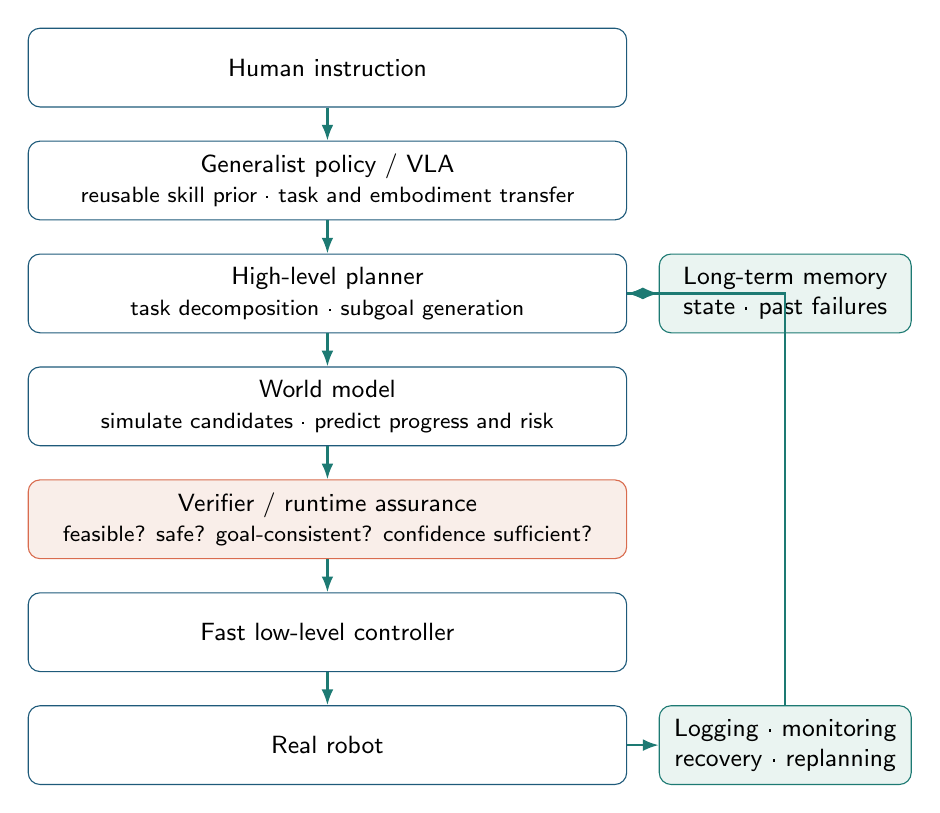
\begin{tikzpicture}[
  node distance=4.2mm,
  every node/.style={font=\sffamily\small,align=center},
  main/.style={draw=midblue,fill=white,rounded corners=1.5mm,minimum width=76mm,minimum height=10mm},
  side/.style={draw=teal,fill=paleteal,rounded corners=1.5mm,minimum width=32mm,minimum height=10mm},
  gate/.style={draw=coral,fill=palecoral,rounded corners=1.5mm,minimum width=76mm,minimum height=10mm},
  arr/.style={-{Latex[length=2mm]},thick,color=teal}
]
\node[main] (human) {Human instruction};
\node[main,below=of human] (vla) {Generalist policy / VLA\\{\footnotesize reusable skill prior · task and embodiment transfer}};
\node[main,below=of vla] (plan) {High-level planner\\{\footnotesize task decomposition · subgoal generation}};
\node[side,right=4mm of plan] (memory) {Long-term memory\\state · past failures};
\node[main,below=of plan] (world) {World model\\{\footnotesize simulate candidates · predict progress and risk}};
\node[gate,below=of world] (verify) {Verifier / runtime assurance\\{\footnotesize feasible? safe? goal-consistent? confidence sufficient?}};
\node[main,below=of verify] (control) {Fast low-level controller};
\node[main,below=of control] (robot) {Real robot};
\node[side,right=4mm of robot] (ops) {Logging · monitoring\\recovery · replanning};
\draw[arr] (human) -- (vla);
\draw[arr] (vla) -- (plan);
\draw[arr] (plan) -- (world);
\draw[arr] (world) -- (verify);
\draw[arr] (verify) -- (control);
\draw[arr] (control) -- (robot);
\draw[arr] (plan) -- (memory);
\draw[arr] (memory) -- (plan);
\draw[arr] (robot) -- (ops);
\draw[arr] (ops) |- (plan);
\end{tikzpicture}
\par\medskip
\small 새 조합을 해석하는 정책, 미래를 시험하는 월드모델, 상태를 유지하는 메모리, 실행을 승인하는 verifier, 실제 성능을 기록하는 평가·assurance가 한 폐루프를 이룹니다.
\end{boardbox}

\begin{profbox}[추가 강의의 결론]
더 큰 VLA 자체가 2026년 중순의 핵심은 아닙니다. 사전학습된 정책을 새 과업과 새 몸에 저비용으로 옮기고, world model로 결과를 미리 시험하며, memory--planner--controller--verifier 구조로 긴 실패를 관리하고, 이를 반복 가능한 실로봇 평가와 assurance 체계로 검증하는 것이 중심 문제로 올라왔습니다.
\end{profbox}

\begin{fieldbox}[다른 발표를 볼 때 던질 다섯 질문]
\begin{enumerate}
  \item 무엇이 실제로 처음 보는 과업 조합이며, 어느 기체까지 이전했는가?
  \item World model이 영상을 만들기만 했는가, 실제 폐루프 결정을 개선했는가?
  \item 누가 상태를 기억하고, 누가 행동을 승인하며, 실패하면 누가 복구하는가?
  \item 몇 번·몇 장소·몇 기체에서 평가했고, 실패의 꼬리와 심각도는 어떠한가?
  \item 모델이 바뀐 뒤에도 안전 주장을 지지하는 시험·로그·rollback 근거가 남는가?
\end{enumerate}
\end{fieldbox}

\cleardoublepage
\part*{핵심 개념 지도}
\addcontentsline{toc}{part}{핵심 개념 지도}

앞의 서사를 다시 찾을 수 있도록 핵심 용어를 시스템 역할별로 정리합니다. 정의를 외우기보다 ``어느 입력을 받아 어떤 책임을 지는가''를 확인하십시오.

\chapter*{정책과 시간척도}
\addcontentsline{toc}{chapter}{핵심 개념: 정책과 시간척도}

\begin{termcard}{Vision-Language-Action}
시각과 언어를 행동으로 연결하는 범용 정책 계열이다. 진짜 가치는 자연어 시연보다 여러 작업과 기체에서 사전학습 자산을 재사용하는 데 있다. 저수준 제어와 안전 권한까지 하나의 모델에 맡길지, specialist와 나눌지가 핵심 설계 질문이다.
\end{termcard}

\begin{termcard}{정책 학습과 제어}
표현 능력을 반복 가능한 물리 행동으로 바꾸는 마지막 계층이다. 의미 정책의 느린 주기와 servo control의 빠른 주기를 연결하며, 지연·진동·접촉 오차·disturbance를 다룬다.
\end{termcard}

\begin{termcard}{Diffusion·flow matching}
여러 가능한 연속 행동 mode를 보존하는 생성형 정책 방식이다. 평균화된 행동을 피하는 대신 iterative sampling과 제어 지연이 생길 수 있어 few-step 생성, action chunking, value guidance가 중요하다.
\end{termcard}

\begin{termcard}{계층적 구조}
mission, subgoal, skill, motor primitive를 서로 다른 시간척도로 나누는 설계다. 계산 절감뿐 아니라 실패 격리와 책임 추적을 가능하게 한다. 계층 경계의 정보 손실과 interface error가 반대편 위험이다.
\end{termcard}

\begin{termcard}{폐루프}
행동 결과를 재관측하고 다음 행동을 수정하는 조건이다. 특정 방법의 이름이라기보다 모든 정책이 실제 환경에서 통과해야 하는 평가 방식이다.
\end{termcard}

\begin{termcard}{Training-free 추론}
가중치 업데이트 없이 검색, scheduling, tool, memory, sampling, verifier로 행동을 개선한다. 버전 관리가 쉬울 수 있지만 계산량과 heuristic 위험은 남는다.
\end{termcard}

\chapter*{세계 상태와 감각}
\addcontentsline{toc}{chapter}{핵심 개념: 세계 상태와 감각}

\begin{termcard}{공간·기하 grounding}
언어와 픽셀을 실제 좌표, 방향, 도달 가능성, 충돌 여유로 고정하는 일이다. ``무엇인가''를 ``어디를 어떻게 행동할 수 있는가''로 바꾼다.
\end{termcard}

\begin{termcard}{3D·BEV·LiDAR 인지}
깊이, 자유 공간, 가림, 상대 속도를 planner가 사용할 수 있는 상태로 만든다. 센서 보정과 동기화 비용이 크며, 명시적 상태와 latent representation의 절충이 있다.
\end{termcard}

\begin{termcard}{Occupancy}
공간을 free, occupied, unknown으로 표현해 물체 종류와 무관하게 충돌과 이동 가능성을 다룬다. semantic·probabilistic·temporal occupancy로 확장될수록 planning의 공유 상태가 된다.
\end{termcard}

\begin{termcard}{의미 표현·semantic modeling}
객체 이름을 기능, affordance, 역할, 관계, task relevance로 확장한다. 의미적 압축은 일반화를 돕지만 접촉과 정밀 기하를 잃지 않도록 해야 한다.
\end{termcard}

\begin{termcard}{촉각·접촉·고유수용감각}
시각으로 보기 어려운 미끄러짐, 힘, 삽입 상태, 관절 위치를 알려준다. contact-rich manipulation의 핵심 feedback channel이지만 센서별 차이와 시간 정렬이 어렵다.
\end{termcard}

\begin{termcard}{멀티모달 학습}
언어, 영상, depth, touch, audio, proprioception, action을 함께 다룬다. modality 수보다 상황별 신뢰도 routing, 결측 센서 강건성, causal alignment가 중요하다.
\end{termcard}

\begin{termcard}{SLAM·지도 구축}
로봇의 위치와 환경 구조를 일관되게 유지한다. 장기 에이전트에서는 localization map을 넘어 semantic·task memory의 좌표계가 되며, 갱신·망각·reset 정책이 필요하다.
\end{termcard}

\begin{termcard}{Gaussian splatting}
장면을 빠르게 렌더링할 수 있는 명시적 3D primitive 표현이다. streaming digital twin과 sensor conversion에 유망하지만 robot-native map이 되려면 dynamics, semantics, uncertainty, collision geometry가 더 필요하다.
\end{termcard}

\chapter*{기억·추론·미래}
\addcontentsline{toc}{chapter}{핵심 개념: 기억·추론·미래}

\begin{termcard}{Memory}
현재 관측에 없는 진행 상태, 이전 행동, 가림 뒤 정보, 실패 경험을 보존한다. 저장량보다 retrieval, update, forgetting, provenance가 중요하다.
\end{termcard}

\begin{termcard}{추론}
상황을 해석하고 도구, 제약, 중간 목표를 선택한다. 자연어 설명의 유창함이 아니라 실행 가능한 predicate, 좌표, 예상 결과와 motor action의 일치로 평가해야 한다.
\end{termcard}

\begin{termcard}{계획}
목표를 행동 순서와 trajectory로 바꾼다. 유연한 learned planner와 보장성이 있는 symbolic·geometric constraint를 receding horizon 안에서 결합하는 것이 현실적인 방향이다.
\end{termcard}

\begin{termcard}{World model}
상태와 행동을 조건으로 미래 관측이나 상태를 예측한다. renderer, simulator, planner를 구분해야 하며, 가치는 시각 품질보다 counterfactual decision과 폐루프 성능 개선으로 입증해야 한다.
\end{termcard}

\begin{termcard}{장기 작업}
여러 단계의 누적 오류, 상태 망각, 단계 전환을 다룬다. 전체 성공률뿐 아니라 checkpoint, partial completion, resume, recovery time이 핵심이다.
\end{termcard}

\begin{termcard}{궤적·동작 예측}
다른 행위자의 여러 가능한 미래를 제공한다. ego action에 따라 상대의 미래도 바뀌므로 joint, interactive, counterfactual distribution과 calibration이 중요하다.
\end{termcard}

\chapter*{몸과 응용}
\addcontentsline{toc}{chapter}{핵심 개념: 몸과 응용}

\begin{termcard}{Embodied AI}
지식을 실제 감각, 행동, 결과 피드백에 접지하는 상위 문제다. 하나의 독립 알고리즘이라기보다 perception--reasoning--action--verification 전체 시스템을 가리킨다.
\end{termcard}

\begin{termcard}{로봇 조작}
VLA, geometry, tactile, planning, recovery를 함께 시험하는 대표 작업군이다. 단순 pick-and-place에서 tool use, assembly, mobile manipulation, household workflow로 범위가 넓어진다.
\end{termcard}

\begin{termcard}{정교 조작·양손·grasping}
작은 기하와 접촉 오차, 높은 자유도, 손 사이 상호작용을 다룬다. task-level policy와 빠른 hand controller, visuo-tactile feedback의 분업이 중요하다.
\end{termcard}

\begin{termcard}{휴머노이드·다족 보행}
이동과 조작이 결합된 whole-body 문제다. 생성형 motion의 화려함보다 균형, 에너지, 낙상 복구, 사람 근접 안전, sim-to-real을 봐야 한다.
\end{termcard}

\begin{termcard}{항법}
단순 목표점 도달에서 언어 목표, semantic map, memory, social interaction, manipulation 전환을 포함한 mission 수행으로 확장된다.
\end{termcard}

\begin{termcard}{자율주행}
대규모 sensor log, rare event, 폐루프 simulation, safety case, fleet update가 결합된 선행 응용이다. learned core와 명시적 safety envelope의 역할 분담이 핵심이다.
\end{termcard}

\begin{termcard}{UAV·공중 로봇}
빠른 3D dynamics, 제한된 compute·battery·통신, 추락 위험을 함께 가진다. 언어 mission planner와 검증된 autopilot의 계층 결합이 현실적이다.
\end{termcard}

\begin{termcard}{Cross-embodiment 전이}
서로 다른 몸 사이에 task semantics와 visual dynamics를 공유한다. 공통 latent action과 기체 adapter가 유망하지만 morphology 차이에서 negative transfer를 측정해야 한다.
\end{termcard}

\begin{termcard}{다중 에이전트·협력}
여러 로봇과 행위자가 역할, map, memory, 자원을 조정한다. 공유량보다 통신 단절, decentralized safety, role conflict, 오류 확산을 다루는 protocol이 중요하다.
\end{termcard}

\chapter*{신뢰성·데이터·운영}
\addcontentsline{toc}{chapter}{핵심 개념: 신뢰성·데이터·운영}

\begin{termcard}{강건성·일반화}
환경 변화와 분포 이동에서 성능이 어떻게 무너지는지 다룬다. 변화 축을 분해하고 uncertainty, abstention, shift detection, bounded adaptation을 함께 평가한다.
\end{termcard}

\begin{termcard}{효율화·압축}
지연, 메모리, 에너지, token, sampling step을 줄여 제어 주기와 edge budget을 맞춘다. 모델 하나의 크기보다 sensor--network--hardware 공동 설계가 중요하다.
\end{termcard}

\begin{termcard}{벤치마크·평가}
가능성을 검증 가능한 주장으로 바꾼다. task success 외에 장기성, 안전, intervention, recovery, throughput, uncertainty와 독립 평가 조건이 필요하다.
\end{termcard}

\begin{termcard}{안전·위험}
위험 인식뿐 아니라 행동 차단, 속도·힘 제한, human override, event log, safety case, 사후 모니터링을 포함하는 실행 보증 구조다.
\end{termcard}

\begin{termcard}{실패 이해·복구·보정}
실패를 detection, diagnosis, repair, escalation으로 나눈다. 실패를 0으로 만드는 것보다 recoverability와 mean time to recovery가 운영가치를 좌우할 수 있다.
\end{termcard}

\begin{termcard}{생성·시뮬레이션}
실제 데이터가 부족한 희귀 상황과 counterfactual을 통제해 만든다. 시각 품질보다 물리·인과 타당성과 실제 policy improvement를 검증해야 한다.
\end{termcard}

\begin{termcard}{인간 선호·시연}
정답 행동, 언어 coaching, 결과 선호, intervention을 통해 작업 기준을 전달한다. 신호마다 비용과 편향이 다르며 reward hacking과 evaluator inconsistency를 살펴야 한다.
\end{termcard}

\begin{termcard}{Zero-shot 일반화}
새 데이터 없이 새로운 조건에 적응하는 능력이다. object, scene, task composition, dynamics, sensor, embodiment를 구분하고 refusal과 recovery까지 평가해야 한다.
\end{termcard}

\begin{termcard}{데이터 수집·증강}
실로봇 로그, 인간 영상, 합성 sensor data, 실패 trace를 연결한다. 양보다 품질 filtering, provenance, license, 실패 coverage, 실세계 재검증이 중요하다.
\end{termcard}

\begin{termcard}{온라인 적응·지속 학습}
배포 후 변한 환경에서 policy, adapter, memory, skill을 갱신한다. full-model update보다 bounded change, shadow evaluation, versioning, rollback이 현실적인 후보 패턴이다.
\end{termcard}

\cleardoublepage
\backmatter
\chapter*{더 읽을 거리}
\addcontentsline{toc}{chapter}{더 읽을 거리}

아래 자료는 이 책의 기술적 배경과 2026년까지의 공개 사례를 확인할 수 있는 출발점이다. 기업 연구 발표와 사전공개 연구는 해당 팀이 보고한 결과로 읽어야 하며, 독립 재현과 분야 전체의 보편적 성능을 뜻하지 않는다.

\section*{추가 강의의 직접 근거}

\sourceitem{CrossFormer: Scaling Cross-Embodied Learning}
{여러 robot embodiment의 데이터를 하나의 정책으로 학습해 기체 간 전이를 다룬 연구.}
{https://proceedings.mlr.press/v270/doshi25a.html}

\sourceitem{LAP: Language-Action Pre-Training}
{언어 형식의 저수준 행동 표현을 이용한 zero-shot cross-embodiment transfer 사전공개 연구.}
{https://arxiv.org/abs/2602.10556}

\sourceitem{DINO-WM}
{Pretrained visual feature의 미래를 예측하고 목표 feature에 맞는 action sequence를 최적화하는 planning 연구.}
{https://proceedings.mlr.press/v267/zhou25t.html}

\sourceitem{WorldGym (formerly Evaluating Robot Policies in a World Model)}
{Action-conditioned video model의 Monte Carlo rollout으로 정책 순위를 추정하는 연구.}
{https://arxiv.org/abs/2506.00613}

\sourceitem{HAVE: History-Aware Verifier}
{행동 생성과 과거 상호작용을 이용한 후보 행동 검증을 분리한 연구.}
{https://proceedings.mlr.press/v305/li25e.html}

\sourceitem{HELM}
{장기 과업의 memory, verification, recovery gap을 모듈로 분해한 사전공개 연구.}
{https://arxiv.org/abs/2604.18791}

\sourceitem{AutoEval}
{Success detection과 scene reset을 자동화해 실제 로봇 정책을 반복 평가하는 연구.}
{https://arxiv.org/html/2503.24278v1}

\sourceitem{ISO 10218-1:2025}
{산업용 로봇 자체의 안전 설계와 위험 저감 요구사항.}
{https://www.iso.org/standard/73933.html}

\sourceitem{Navigating the AI Act}
{EU AI Act의 분류와 요구사항을 설명하는 유럽연합 공식 안내.}
{https://digital-strategy.ec.europa.eu/en/faqs/navigating-ai-act}

\section*{본문의 공개 자료}

\sourceitem{π0.7: A Steerable Model with Emergent Capabilities}
{새 과업 조합, 기체 전이, visual subgoal을 포함한 범용 정책 사례.}
{https://www.pi.website/blog/pi07}

\sourceitem{Gemini Robotics-ER 1.6}
{공간 추론, tool calling, 물리적 제약을 다루는 embodied reasoner 사례.}
{https://deepmind.google/blog/gemini-robotics-er-1-6/}

\sourceitem{Cosmos 3}
{text, image, video, audio, action과 forward·inverse dynamics를 함께 다루는 월드모델 연구.}
{https://research.nvidia.com/labs/cosmos-lab/cosmos3/}

\sourceitem{Vesta}
{localization, navigation, reasoning, planning을 통합한 embodied planner.}
{https://research.nvidia.com/labs/gear/vesta/}

\sourceitem{Multi-Scale Embodied Memory}
{영상 단기 기억과 언어 장기 기억을 분리한 장기 로봇 작업 연구.}
{https://www.pi.website/research/memory}

\sourceitem{RL Token: Precise Manipulation with Efficient Online RL}
{frozen VLA의 표현을 작은 actor와 critic의 현장 보정에 이용한 사례.}
{https://www.pi.website/research/rlt}

\sourceitem{ASPIRE}
{multimodal execution trace, 반복 디버깅, 지속되는 skill library를 다룬 연구.}
{https://research.nvidia.com/labs/gear/aspire/}

\sourceitem{EgoScale}
{대규모 인간 egocentric video와 정교 조작 전이를 다룬 연구.}
{https://research.nvidia.com/labs/gear/egoscale/}

\sourceitem{The Waymo World Model}
{희귀 주행 상황과 multi-sensor rollout을 생성하는 자율주행 월드모델 사례.}
{https://waymo.com/blog/2026/02/the-waymo-world-model-a-new-frontier-for-autonomous-driving-simulation/}

\sourceitem{Sensor2Sensor}
{외부 monocular video를 multi-view camera와 LiDAR 형태로 변환하는 sensor simulation 연구.}
{https://waymo.com/research/sensor-2-sensor-cross-embodiment-sensor/}

\sourceitem{Waymo 6th-generation Driver}
{센서 수, redundancy, custom compute의 시스템 공동 설계를 볼 수 있는 공개 자료.}
{https://waymo.com/blog/2026/02/ro-on-6th-gen-waymo-driver/}

\sourceitem{RoboArena}
{여러 기관의 실제 로봇을 이용한 분산·비교 평가 프로토콜.}
{https://robo-arena.github.io/}

\sourceitem{BEHAVIOR-1K}
{현실적인 장기 일상 작업과 full-task 평가를 다루는 benchmark.}
{https://behavior.stanford.edu/index.html}

\sourceitem{VLA-Arena}
{안전, distractor, extrapolation, long-horizon을 분리해 평가하는 환경.}
{https://vla-arena.github.io/}

\sourceitem{ISO 10218-2:2025}
{산업용 로봇 application과 cell의 integration, operation, maintenance 안전 요구.}
{https://www.iso.org/standard/73934.html}

\sourceitem{EU AI Act official timeline}
{2026년 7월 24일 갱신된 유럽연합 공식 적용 일정. 규제 제품에 내장된 high-risk AI 규칙은 2028년 8월 2일부터 적용된다고 설명한다.}
{https://digital-strategy.ec.europa.eu/en/policies/regulatory-framework-ai}

\sourceitem{Regulation (EU) 2026/1744}
{EU AI Act의 적용 일정을 개정한 2026년 7월 공표 규정 원문.}
{https://eur-lex.europa.eu/eli/reg/2026/1744/oj}

\sourceitem{Do What You Say}
{언어 계획과 motor action의 불일치를 runtime reasoning과 verification으로 다룬 연구.}
{https://research.nvidia.com/publication/2026-06_do-what-you-say-steering-vision-language-action-models-runtime-reasoning-action}

\sourceitem{FAST}
{연속 robot action을 압축하는 action tokenization 연구.}
{https://www.pi.website/research/fast}

\sourceitem{Real-Time Action Chunking}
{대형 정책의 추론 중에도 계속 변하는 세계에서 비동기 행동을 연결하는 방법.}
{https://www.pi.website/research/real_time_chunking}

\sourceitem{Gemini Robotics On-Device}
{낮은 지연과 network-independent 실행을 겨냥한 on-device 로봇 모델 사례.}
{https://deepmind.google/blog/gemini-robotics-on-device-brings-ai-to-local-robotic-devices/}

\sourceitem{Sparsh}
{대규모 자기지도 촉각 표현과 여러 tactile sensor·task를 다룬 연구.}
{https://ai.meta.com/research/publications/sparsh-self-supervised-touch-representations-for-vision-based-tactile-sensing/}

\sourceitem{Diffusion Policy}
{다봉성 연속 행동과 receding-horizon control에 diffusion을 적용한 기초 연구.}
{https://diffusion-policy.cs.columbia.edu/}

\sourceitem{Spark 2.0}
{대규모 3D Gaussian splatting 세계의 streaming과 level-of-detail 사례.}
{https://www.worldlabs.ai/blog/spark-2.0}

\sourceitem{LoopSplat}
{3D Gaussian submap의 online loop closure와 global consistency 연구.}
{https://www.research-collection.ethz.ch/items/1a129549-57a5-4cb7-abcc-148920c202c1}

\sourceitem{Uni-LaViRA}
{여러 navigation task와 embodiment를 하나의 agent loop로 다루는 사전공개 연구.}
{https://arxiv.org/abs/2605.27582}

\sourceitem{WorldFly}
{도시 환경 UAV에서 미래 video와 action을 함께 생성하는 사전공개 연구.}
{https://arxiv.org/abs/2606.06147}

\sourceitem{GR00T N1.6}
{여러 로봇 기체의 bimanual과 loco-manipulation을 다루는 공개 모델 자료.}
{https://research.nvidia.com/labs/gear/gr00t-n1_6/}

\sourceitem{GRAIL}
{3D asset와 video prior로 whole-body sequence를 생성하고 실기체로 옮기는 연구.}
{https://research.nvidia.com/labs/dair/grail/}

\sourceitem{Open X-Embodiment}
{여러 embodiment의 robot trajectory를 모은 초기 대규모 데이터 협력.}
{https://robotics-transformer-x.github.io/}

\sourceitem{Hi Robot}
{고수준 VLM과 저수준 VLA, 인간 interjection을 결합한 계층형 정책.}
{https://www.pi.website/research/hirobot}

\sourceitem{AutoRT}
{여러 로봇의 대규모 데이터 수집과 fleet orchestration을 다룬 연구.}
{https://deepmind.google/research/publications/48151/}

\sourceitem{GenDP}
{3D semantic field와 diffusion policy를 결합한 unseen-instance 조작 연구.}
{https://robopil.github.io/GenDP/}

\sourceitem{UniScene}
{semantic occupancy를 중심으로 video와 LiDAR 생성을 통합한 driving scene pipeline.}
{https://cvpr.thecvf.com/virtual/2025/poster/32687}

\sourceitem{A Functional Taxonomy of World Models}
{renderer, simulator, planner와 그 사이의 loop를 구분하는 개념 틀. 합의된 표준 정의라기보다 유용한 분석 프레임으로 읽는다.}
{https://www.worldlabs.ai/blog/taxonomy-of-world-models}

\cleardoublepage
\thispagestyle{empty}
\vspace*{\fill}
\begin{center}
{\sffamily\bfseries\Large\color{deepblue}2026 하반기 Physical AI 동향}\par
\vspace{6mm}
{\color{coral}\rule{35mm}{1.5pt}}\par
\vspace{6mm}
{\small
2026년 7월 26일까지 공개적으로 확인 가능한 자료를 바탕으로 작성한 분석적 해설이다.\par
전망은 확정 사실이 아니며, 실제 안전·규정·제품 판단은 용도별 검증이 필요하다.}
\end{center}
\vspace*{\fill}

\end{document}
